%  LaTeX support: latex@mdpi.com 
%  For support, please attach all files needed for compiling as well as the log file, and specify your operating system, LaTeX version, and LaTeX editor.


%=================================================================
\documentclass[agriengineering,article,submit,pdftex,moreauthors]{Definitions/mdpi} 
%\documentclass[journal,article,submit,pdftex,moreauthors]{Definitions/mdpi} 


%\documentclass[preprints,article,submit,pdftex,moreauthors]{Definitions/mdpi} 
% For posting an early version of this manuscript as a preprint, you may use "preprints" as the journal. Changing "submit" to "accept" before posting will remove line numbers.

% Below journals will use APA reference format:
% admsci, behavsci, businesses, econometrics, economies, education, ejihpe, games, humans, ijfs, journalmedia, jrfm, languages, psycholint, publications, tourismhosp, youth

% Below journals will use Chicago reference format:
% arts, genealogy, histories, humanities, jintelligence, laws, literature, religions, risks, socsci

%--------------------
% Class Options:
%--------------------
%----------
% journal
%----------
% Choose between the following MDPI journals:
% accountaudit, acoustics, actuators, addictions, adhesives, admsci, adolescents, aerobiology, aerospace, agriculture, agriengineering, agrochemicals, agronomy, ai, air, algorithms, allergies, alloys, amh, analytica, analytics, anatomia, anesthres, animals, antibiotics, antibodies, antioxidants, applbiosci, appliedchem, appliedmath, appliedphys, applmech, applmicrobiol, applnano, applsci, aquacj, architecture, arm, arthropoda, arts, asc, asi, astronomy, atmosphere, atoms, audiolres, automation, axioms, bacteria, batteries, bdcc, behavsci, beverages, biochem, bioengineering, biologics, biology, biomass, biomechanics, biomed, biomedicines, biomedinformatics, biomimetics, biomolecules, biophysica, biosensors, biosphere, biotech, birds, blockchains, bloods, blsf, brainsci, breath, buildings, businesses, cancers, carbon, cardiogenetics, catalysts, cells, ceramics, challenges, chemengineering, chemistry, chemosensors, chemproc, children, chips, cimb, civileng, cleantechnol, climate, clinbioenerg, clinpract, clockssleep, cmd, cmtr, coasts, coatings, colloids, colorants, commodities, complications, compounds, computation, computers, condensedmatter, conservation, constrmater, cosmetics, covid, crops, cryo, cryptography, crystals, csmf, ctn, curroncol, cyber, dairy, data, ddc, dentistry, dermato, dermatopathology, designs, devices, diabetology, diagnostics, dietetics, digital, disabilities, diseases, diversity, dna, drones, dynamics, earth, ebj, ecm, ecologies, econometrics, economies, education, eesp, ejihpe, electricity, electrochem, electronicmat, electronics, encyclopedia, endocrines, energies, eng, engproc, ent, entomology, entropy, environments, epidemiologia, epigenomes, esa, est, famsci, fermentation, fibers, fintech, fire, fishes, fluids, foods, forecasting, forensicsci, forests, fossstud, foundations, fractalfract, fuels, future, futureinternet, futureparasites, futurepharmacol, futurephys, futuretransp, galaxies, games, gases, gastroent, gastrointestdisord, gastronomy, gels, genealogy, genes, geographies, geohazards, geomatics, geometry, geosciences, geotechnics, geriatrics, glacies, grasses, greenhealth, gucdd, hardware, hazardousmatters, healthcare, hearts, hemato, hematolrep, heritage, higheredu, highthroughput, histories, horticulturae, hospitals, humanities, humans, hydrobiology, hydrogen, hydrology, hygiene, idr, iic, ijerph, ijfs, ijgi, ijmd, ijms, ijns, ijpb, ijt, ijtm, ijtpp, ime, immuno, informatics, information, infrastructures, inorganics, insects, instruments, inventions, iot, j, jal, jcdd, jcm, jcp, jcs, jcto, jdad, jdb, jeta, jfb, jfmk, jimaging, jintelligence, jlpea, jmahp, jmmp, jmms, jmp, jmse, jne, jnt, jof, joitmc, joma, jop, jor, journalmedia, jox, jpbi, jpm, jrfm, jsan, jtaer, jvd, jzbg, kidney, kidneydial, kinasesphosphatases, knowledge, labmed, laboratories, land, languages, laws, life, lights, limnolrev, lipidology, liquids, literature, livers, logics, logistics, lubricants, lymphatics, machines, macromol, magnetism, magnetochemistry, make, marinedrugs, materials, materproc, mathematics, mca, measurements, medicina, medicines, medsci, membranes, merits, metabolites, metals, meteorology, methane, metrics, metrology, micro, microarrays, microbiolres, microelectronics, micromachines, microorganisms, microplastics, microwave, minerals, mining, mmphys, modelling, molbank, molecules, mps, msf, mti, multimedia, muscles, nanoenergyadv, nanomanufacturing, nanomaterials, ncrna, ndt, network, neuroglia, neurolint, neurosci, nitrogen, notspecified, nri, nursrep, nutraceuticals, nutrients, obesities, oceans, ohbm, onco, oncopathology, optics, oral, organics, organoids, osteology, oxygen, parasites, parasitologia, particles, pathogens, pathophysiology, pediatrrep, pets, pharmaceuticals, pharmaceutics, pharmacoepidemiology, pharmacy, philosophies, photochem, photonics, phycology, physchem, physics, physiologia, plants, plasma, platforms, pollutants, polymers, polysaccharides, populations, poultry, powders, preprints, proceedings, processes, prosthesis, proteomes, psf, psych, psychiatryint, psychoactives, psycholint, publications, purification, quantumrep, quaternary, qubs, radiation, reactions, realestate, receptors, recycling, regeneration, religions, remotesensing, reports, reprodmed, resources, rheumato, risks, robotics, rsee, ruminants, safety, sci, scipharm, sclerosis, seeds, sensors, separations, sexes, signals, sinusitis, siuj, skins, smartcities, sna, societies, socsci, software, soilsystems, solar, solids, spectroscj, sports, standards, stats, std, stresses, surfaces, surgeries, suschem, sustainability, symmetry, synbio, systems, tae, targets, taxonomy, technologies, telecom, test, textiles, thalassrep, therapeutics, thermo, timespace, tomography, tourismhosp, toxics, toxins, transplantology, transportation, traumacare, traumas, tropicalmed, universe, urbansci, uro, vaccines, vehicles, venereology, vetsci, vibration, virtualworlds, viruses, vision, waste, water, wem, wevj, wild, wind, women, world, youth, zoonoticdis

%---------
% article
%---------
% The default type of manuscript is "article", but can be replaced by: 
% abstract, addendum, article, benchmark, book, bookreview, briefcommunication, briefreport, casereport, changes, clinicopathologicalchallenge, comment, commentary, communication, conceptpaper, conferenceproceedings, correction, conferencereport, creative, datadescriptor, discussion, entry, expressionofconcern, extendedabstract, editorial, essay, erratum, fieldguide, hypothesis, interestingimages, letter, meetingreport, monograph, newbookreceived, obituary, opinion, proceedingpaper, projectreport, reply, retraction, review, perspective, protocol, shortnote, studyprotocol, supfile, systematicreview, technicalnote, viewpoint, guidelines, registeredreport, tutorial,  giantsinurology, urologyaroundtheworld
% supfile = supplementary materials

%----------
% submit
%----------
% The class option "submit" will be changed to "accept" by the Editorial Office when the paper is accepted. This will only make changes to the frontpage (e.g., the logo of the journal will get visible), the headings, and the copyright information. Also, line numbering will be removed. Journal info and pagination for accepted papers will also be assigned by the Editorial Office.

%------------------
% moreauthors
%------------------
% If there is only one author the class option oneauthor should be used. Otherwise use the class option moreauthors.

%---------
% pdftex
%---------
% The option pdftex is for use with pdfLaTeX. Remove "pdftex" for (1) compiling with LaTeX & dvi2pdf (if eps figures are used) or for (2) compiling with XeLaTeX.

%=================================================================
% MDPI internal commands - do not modify
\firstpage{1} 
\makeatletter 
\setcounter{page}{\@firstpage} 
\makeatother
\pubvolume{1}
\issuenum{1}
\articlenumber{0}
\pubyear{2025}
\copyrightyear{2024}
%\externaleditor{Firstname Lastname} % More than 1 editor, please add `` and '' before the last editor name
\datereceived{ } 
\daterevised{ } % Comment out if no revised date
\dateaccepted{ } 
\datepublished{ } 
%\datecorrected{} % For corrected papers: "Corrected: XXX" date in the original paper.
%\dateretracted{} % For retracted papers: "Retracted: XXX" date in the original paper.
\hreflink{https://doi.org/} % If needed use \linebreak
%\doinum{}
%\pdfoutput=1 % Uncommented for upload to arXiv.org
%\CorrStatement{yes}  % For updates
%\longauthorlist{yes} % For many authors that exceed the left citation part

%=================================================================
% Add packages and commands here. The following packages are loaded in our class file: fontenc, inputenc, calc, indentfirst, fancyhdr, graphicx, epstopdf, lastpage, ifthen, float, amsmath, amssymb, lineno, setspace, enumitem, mathpazo, booktabs, titlesec, etoolbox, tabto, xcolor, colortbl, soul, multirow, microtype, tikz, totcount, changepage, attrib, upgreek, array, tabularx, pbox, ragged2e, tocloft, marginnote, marginfix, enotez, amsthm, natbib, hyperref, cleveref, scrextend, url, geometry, newfloat, caption, draftwatermark, seqsplit
% cleveref: load \crefname definitions after \begin{document}

% BEM ADDITIONS BEGIN
\usepackage{longtable}
\usepackage{amsmath}

% BEM ADDITIONS END

%=================================================================
% Please use the following mathematics environments: Theorem, Lemma, Corollary, Proposition, Characterization, Property, Problem, Example, ExamplesandDefinitions, Hypothesis, Remark, Definition, Notation, Assumption
%% For proofs, please use the proof environment (the amsthm package is loaded by the MDPI class).

%=================================================================
% Full title of the paper (Capitalized)
\Title{Class Imbalance in Crop/Weed Classification}

% MDPI internal command: Title for citation in the left column
\TitleCitation{Class Imbalance in Crop/Weed Classification}

% Author Orchid ID: enter ID or remove command
\newcommand{\orcidauthorA}{0009-0002-3582-2576} % Add \orcidA{} behind the author's name
%\newcommand{\orcidauthorB}{0000-0000-0000-000X} % Add \orcidB{} behind the author's name

% Authors, for the paper (add full first names)
%\Author{Evan McGinnis $^{1,\dagger,\ddagger}$\orcidA{}, Firstname Lastname $^{2,\ddagger}$ and Firstname Lastname $^{2,}$*}
\Author{Brian E McGinnis $^{1,\dagger,\ddagger}$\orcidA{}}

%\longauthorlist{yes}

% MDPI internal command: Authors, for metadata in PDF
\AuthorNames{\orcidA Brian E McGinnis}

% MDPI internal command: Authors, for citation in the left column, only choose below one of them according to the journal style
% If this is a Chicago style journal: Lastname, Firstname, Firstname Lastname, and Firstname Lastname.
% If this is a APA style journal: Lastname, F., Lastname, F., \& Lastname, F.
% If this is a ACS style journal: Lastname, F.; Lastname, F.; Lastname, F.
%\isAPAStyle{%
%       \AuthorCitation{McGinnis, E., Lastname, F., \& Lastname, F.}
%         }{%
%        \isChicagoStyle{%
%        \AuthorCitation{McGinnis, E, Firstname Lastname, and Firstname Lastname.}
%        }{
%        \AuthorCitation{McGinnis, E.; Lastname, F.; Lastname, F.}
%        }
%}

\isAPAStyle{%
       \AuthorCitation{McGinnis, B.}
         }{%
        \isChicagoStyle{%
        \AuthorCitation{McGinnis, B}
        }{
        \AuthorCitation{McGinnis, B.}
        }
}

% Affiliations / Addresses (Add [1] after \address if there is only one affiliation.)
\address{%
$^{1}$ \quad Affiliation 1; evanmc@arizona.edu\\
}
%$^{2}$ \quad Affiliation 2; e-mail@e-mail.com}

% Contact information of the corresponding author
\corres{Correspondence: evanmc@arizona.edu}

% Current address and/or shared authorship
\firstnote{Current address: University of Arizona, Tucson, AZ 85721.}  % Current address should not be the same as any items in the Affiliation section.
\secondnote{These authors contributed equally to this work.}
% The commands \thirdnote{} till \eighthnote{} are available for further notes

%\simplesumm{} % Simple summary

%\conference{} % An extended version of a conference paper

% Abstract (Do not insert blank lines, i.e. \\) 
\abstract{Class imbalance is a common challenge in machine learning for agriculture, where images often contain many more crop plants than weeds. This paper presents an in-depth study of two strategies to address this imbalance in crop/weed classification: (1) oversampling the minority class by generating synthetic data (using algorithms such as SMOTE, Borderline-SMOTE, ADASYN, KMeans-SMOTE, and SVM-SMOTE), and (2) a combined approach of oversampling the minority class and undersampling the majority class (using SMOTE with Tomek links and SMOTE with Edited Nearest Neighbors). We evaluate these strategies on a dataset of segmented crop and weed instances, using multiple classification models: Decision Tree, k-Nearest Neighbors (KNN), Logistic Regression, Multi-Layer Perceptron (MLP), Random Forest, Linear Discriminant Analysis (LDA), Extra Trees, Gradient Boosting, and Support Vector Machine (SVM). Results show that oversampling the weed class generally improves classifier performance (as measured by Area Under the ROC Curve, AUC) compared to no correction, but the magnitude of improvement is often modest. The Decision Tree classifier benefited the most from imbalance correction, with notable AUC gains, whereas an ensemble method like Random Forest often degraded in performance when synthetic data were introduced. Combined over/under-sampling methods further boosted Decision Tree performance but could negatively impact other models (for example, SMOTE+ENN greatly reduced Logistic Regression accuracy, and SMOTE+Tomek slightly harmed Random Forest). We discuss the statistical significance of these improvements, the generalizability of models trained with synthetic data, and practical implications for field deployment. New sections on related work, feature engineering, and limitations are included to provide context and guide future research. We conclude with recommendations for practitioners on when imbalance correction is worthwhile and suggest directions for future work, such as integrating these techniques with deep learning models and using UAV imagery for broader applicability.}

% Keywords
\keyword{imbalance, SMOTE, SVM, KNN, LDA, ENN, Tomek Links, over-sampling, under-sampling} 

% The fields PACS, MSC, and JEL may be left empty or commented out if not applicable
%\PACS{J0101}
%\MSC{}
%\JEL{}

%%%%%%%%%%%%%%%%%%%%%%%%%%%%%%%%%%%%%%%%%%
% Only for the journal Diversity
%\LSID{\url{http://}}

%%%%%%%%%%%%%%%%%%%%%%%%%%%%%%%%%%%%%%%%%%
% Only for the journal Applied Sciences
%\featuredapplication{Authors are encouraged to provide a concise description of the specific application or a potential application of the work. This section is not mandatory.}
%%%%%%%%%%%%%%%%%%%%%%%%%%%%%%%%%%%%%%%%%%

%%%%%%%%%%%%%%%%%%%%%%%%%%%%%%%%%%%%%%%%%%
% Only for the journal Data
%\dataset{DOI number or link to the deposited data set if the data set is published separately. If the data set shall be published as a supplement to this paper, this field will be filled by the journal editors. In this case, please submit the data set as a supplement.}
%\datasetlicense{License under which the data set is made available (CC0, CC-BY, CC-BY-SA, CC-BY-NC, etc.)}

%%%%%%%%%%%%%%%%%%%%%%%%%%%%%%%%%%%%%%%%%%
% Only for the journal Toxins
%\keycontribution{The breakthroughs or highlights of the manuscript. Authors can write one or two sentences to describe the most important part of the paper.}

%%%%%%%%%%%%%%%%%%%%%%%%%%%%%%%%%%%%%%%%%%
% Only for the journal Encyclopedia
%\encyclopediadef{For entry manuscripts only: please provide a brief overview of the entry title instead of an abstract.}

%%%%%%%%%%%%%%%%%%%%%%%%%%%%%%%%%%%%%%%%%%
% Only for the journal Advances in Respiratory Medicine and Smart Cities
%\addhighlights{yes}
%\renewcommand{\addhighlights}{%

%\noindent This is an obligatory section in “Advances in Respiratory Medicine'' and ``Smart Cities”, whose goal is to increase the discoverability and readability of the article via search engines and other scholars. Highlights should not be a copy of the abstract, but a simple text allowing the reader to quickly and simplified find out what the article is about and what can be cited from it. Each of these parts should be devoted up to 2~bullet points.\vspace{3pt}\\
%\textbf{What are the main findings?}
% \begin{itemize}[labelsep=2.5mm,topsep=-3pt]
% \item First bullet.
% \item Second bullet.
% \end{itemize}\vspace{3pt}
%\textbf{What is the implication of the main finding?}
% \begin{itemize}[labelsep=2.5mm,topsep=-3pt]
% \item First bullet.
% \item Second bullet.
% \end{itemize}
%}

%%%%%%%%%%%%%%%%%%%%%%%%%%%%%%%%%%%%%%%%%%
\begin{document}

%%%%%%%%%%%%%%%%%%%%%%%%%%%%%%%%%%%%%%%%%%
%\setcounter{section}{-1} %% Remove this when starting to work on the template.
%\section{How to Use this Template}
%
%The template details the sections that can be used in a manuscript. Note that the order and names of article sections may differ from the requirements of the journal (e.g., the positioning of the Materials and Methods section). Please check the instructions on the authors' page of the journal to verify the correct order and names. For any questions, please contact the editorial office of the journal or support@mdpi.com. For LaTeX-related questions please contact latex@mdpi.com.%\endnote{This is an endnote.} % To use endnotes, please un-comment \printendnotes below (before References). Only journal Laws uses \footnote.

% The order of the section titles is different for some journals. Please refer to the "Instructions for Authors” on the journal homepage.


%
%
\section{Introduction}
Precision agriculture often relies on accurate identification of weeds versus crops in field imagery to enable site-specific weed management. Weeds, being undesired plants, typically appear in much smaller quantities than crop plants in a field. From a grower’s perspective this is good – a well-maintained field has few weeds – but from a machine learning perspective it poses a serious challenge: training data for weed recognition are scarce relative to crop data. Overhead images of crop fields usually contain predominantly crop plants with only a few weed instances. For example, if an image dataset contains 100 plants of which only 5 are weeds, a classifier could naively achieve 95\% accuracy by labeling everything as “crop.” This high accuracy is misleading because the model would completely fail to detect weeds, which are the minority class of greatest interest. In extreme cases, an image set might have a ratio of 1000 crops for every weed, or even contain some weed species only in the test set but not in training – making it impossible for the model to learn those weeds. Clearly, class imbalance can bias models toward the majority class (crops) and undermine weed detection performance

Class imbalance is not unique to weed detection; it is a widespread issue in machine learning applications ranging from medical diagnosis to fraud detection. In the context of agriculture, class imbalance often arises due to the rarity of certain events or classes – for instance, images of crops may rarely contain weeds (as in our case) or only a small fraction of plants might show a particular disease or stress condition \cite{Miftahushudur2025-dc}. If left unaddressed, models trained on imbalanced data become biased toward predicting the majority class, failing to generalize to minority class examples.  Moreover, evaluating model performance solely by overall accuracy is inadequate under imbalance, since a high accuracy can be achieved by ignoring the minority class entirely. Metrics like recall, precision, $F_{1}$, and AUC (Area Under the ROC Curve) are preferred to assess performance on imbalanced datasets.

To mitigate class imbalance, two broad categories of solutions exist: data-level methods and algorithm-level methods.  Data-level methods adjust the training data distribution to balance classes, either by oversampling the minority class or undersampling the majority class (or both). Algorithm-level methods modify the learning algorithm to reduce bias toward the majority, for example by using class weightings, adjusted loss functions (e.g., focal loss in deep learning), or specialized architectures. In this work, we focus on data-level approaches, as they are model-agnostic and relatively easy to implement with existing tools. In particular, we examine a range of oversampling techniques that generate synthetic minority samples to augment weed data, as well as combined methods that also perform targeted removal of certain majority (crop) samples. These techniques have been widely discussed in the class-imbalance literature and are supported by libraries such as imbalanced-learn. Our goal is to evaluate their efficacy in a real crop/weed classification task and provide guidance on their usage in agricultural applications.

%
This paper is organized as follows. In Section \ref{section:related}, we review prior research on class imbalance in plant phenotyping and agricultural classification, including both classical machine learning and deep learning approaches. Section \ref{section:materials} describes our dataset of crop and weed images, the preprocessing and feature engineering pipeline used to extract quantitative features from plants, and the methodology of applying various oversampling and undersampling algorithms. We detail the specific algorithms (SMOTE variants, Tomek links, Edited Nearest Neighbors) in subsections for clarity. Section \ref{section:results} presents the performance of several classifiers on imbalanced vs. balanced training data, comparing metrics like AUC, precision, and recall. We visualize the impact of imbalance correction through ROC curves and AUC change plots. Section \ref{section:discussion} provides an analysis of the results, including statistical considerations, why certain models reacted differently to imbalance correction, and practical implications for using these techniques. In Section 6 (Limitations), we discuss the constraints and assumptions of our study – such as the realism of synthetic data and generalizability beyond our dataset. Finally, Section \ref{section:conclusion} summarizes the key findings and contributions, and outlines future research directions, including integration with deep learning and the use of UAV (Unmanned Aerial Vehicle) imagery to extend this work.
%
\section{Related Work}
\label{section:related}
Class imbalance is prevalent in agricultural datasets and has received increasing attention in recent years.  A recent survey by Miftahushudur et al. (2025) provides a comprehensive review of imbalance issues in precision agriculture, covering plant disease detection, soil condition classification, and crop/weed discrimination \cite{Miftahushudur2025-dc}. The survey highlights that agricultural data often suffer from skewed class distributions due to rare events (e.g., uncommon diseases) or practical data collection constraints (e.g., weeds sparsely scattered in fields). Common data-level solutions in agriculture include oversampling minority class instances and undersampling the majority, similar to other domains, while algorithm-level solutions involve cost-sensitive learning or ensemble methods.  A notable emerging trend is the use of generative models (GANs and VAEs) to augment minority class data in agriculture.  For example, Ali-Gombe and Elyan (2019) introduced an approach using a Generative Adversarial Network (GAN) to create synthetic data for minority classes (the MFC-GAN) and demonstrated improved classification performance on imbalanced datasets \cite{Ali-Gombe2019-kr, Miftahushudur2025-dc}. Such generative oversampling could potentially be applied to weed images, although it requires sufficient training data to learn the distribution of the minority class.

Early work on weed vs. crop classification often focused on feature engineering and classical classifiers. Guerrero et al. (2012) used Support Vector Machines to distinguish crop and weed plants in imagery, achieving high accuracy by leveraging shape and texture features  \cite{Guerrero2012-zi}. In those days, class imbalance was typically addressed by careful dataset collection – ensuring a reasonable number of weed samples – or by evaluating models with metrics robust to imbalance (e.g., per-class accuracy). As datasets grew in complexity, researchers began to report imbalance issues more explicitly. For instance, a weed species classification study by Dyrmann et al. (2016) compiled a large dataset of several plant species and noted that some species had far fewer examples, necessitating strategies to handle imbalance \cite{Dyrmann2016-uh}.
%

With the rise of deep learning, many recent weed detection studies have shifted to convolutional neural networks (CNNs) and data augmentation to tackle imbalance. Data augmentation (generating new training images by transformations) is effectively a form of oversampling in image space. Hasan et al. (2023) created a combined weed/crop image dataset from multiple sources and dealt with class imbalance by applying extensive image augmentations (flips, rotations, etc.) to minority classes \cite{Mahmudul-Hasan2023-ap}. This approach balanced the class distribution and improved deep CNN performance, reinforcing that augmenting data can mitigate skewed classes in a manner analogous to synthetic oversampling of features. Indeed, Hasan et al. (2023) found that models like ResNet-50 achieved significantly higher recall for rare weed classes after augmentation and fine-tuning. Similarly, Reedha et al. (2022) addressed imbalance in a UAV-based sugar beet field dataset by upsampling the minority class (off-type beets) fourfold using random flips and rotations \citeauthor{Reedha2022-fp}. By doing so, the minority class constituted ~17\% of the training set (up from a much smaller fraction), leading to balanced performance across classes in a Vision Transformer model.

Some researchers have explored combined oversampling/undersampling and other hybrid techniques in agriculture. Sarkar et al. (2023) evaluated SMOTE+ENN (SMOTE with Edited Nearest Neighbors) in a high-throughput phenotyping task (assessing soybean lodging severity from UAV images). They reported that SMOTE+ENN preprocessing consistently improved classification accuracy and $F_{1}$-scores for multiple classifiers (XGBoost, Random Forest, KNN, ANN), achieving up to 96\% overall accuracy with an ANN classifier on a 4-class lodging classification \cite{Sarkar2023-gy}. This suggests that combined cleaning of majority class noise with minority oversampling can be highly effective in some agricultural scenarios. On the other hand, not all studies have found oversampling beneficial; the effectiveness can depend on the dataset characteristics and classifier used. For example, if the minority class samples are not just few but also very different in nature (e.g., entirely different weed species), simplistic oversampling might not help a model truly generalize to new instances. In such cases, algorithm-level methods like class-weighted training or one-class classifiers might be considered. Cost-sensitive learning, where the model is penalized more for misclassifying a weed than a crop, is another strategy that has seen use in imbalance problems, although we did not explore it in this study. 

%
 In summary, prior work demonstrates a spectrum of techniques to handle class imbalance in plant classification. Oversampling via data augmentation or synthetic instance generation is common and has shown success \cite{Sarkar2023-gy} \cite{Miftahushudur2025-dc}. The contributions of this paper lie in systematically comparing multiple oversampling algorithms and their combination with undersampling in a controlled weed/crop classification experiment, and analyzing their effects on a variety of classifiers. This fills a gap in understanding how classical imbalance correction techniques perform in an agricultural context (most previous agricultural studies test one or two methods at most). Moreover, by focusing on a feature-engineering approach (as opposed to end-to-end deep learning), our work offers insights into when and why these data-level methods work, which can inform their use in future precision agriculture projects or hybrid modeling approaches.
%

%
%
%
%
%
%
%
\section{Materials and Methods}
\label{section:materials}
\subsection{Data Collection and Processing}
Our dataset consists of images captured from a cantaloupe field at the University of Arizona’s Maricopa Agricultural Center (MAC) in Maricopa, AZ (coordinates: $33.0618^\circ N$, $111.9656^\circ W$). The images were taken in late April and early May 2024 using a consumer-grade digital camera (Apple iPhone 14) under natural lighting conditions. To ensure color consistency, we performed color calibration on all images: photographs of a Datacolor SpyderCheckr color chart under the same lighting were used to compute correction curves, and these corrections were applied in Adobe Lightroom to all field images. This step minimized color shifts due to lighting variability (e.g., clouds vs. sun) and ensured that color-based features could be compared across images.

Each image contained multiple plants (either crop or weeds) against a soil background. We applied a segmentation algorithm to isolate individual plant instances. Specifically, we used the Combined Indices 2 approach described by Guerrero et al. to generate a vegetation mask \cite{Guerrero2012-zi}.  This method combines spectral indices (such as excess green, excess red) to differentiate vegetation from soil with high accuracy, producing a binary mask of plant vs. background. Using this mask, we extracted bounding patches for each plant and then manually verified and labeled each plant as “crop” or “weed.” In our dataset, the crop plants are young cantaloupe seedlings, and the weeds are a mix of species common to the area (including pigweed and lambsquarters). A custom labeling tool was developed (in Python with OpenCV) to expedite manual classification of the segmented plant images. The result of this preprocessing was a collection of individual plant images, each labeled as crop or weed
%

Because the original proportion of weeds in the dataset was low (reflecting a well-maintained field), we deliberately created several subsets with varying class imbalance ratios for our experiments. In other words, we simulated scenarios of increasing severity of class imbalance by subsampling the weed instances. For example, suppose the fully segmented dataset initially had a crop:weed ratio of about 5:1 (which is relatively mild imbalance); we randomly dropped weed samples to create more imbalanced training sets such as 10:1, 30:1, and 50:1. In one extreme setting, we retained only 2–3 weed samples against a large number of crops to mimic a highly imbalanced scenario (e.g., 50:1). By preparing multiple versions of the training data with weed counts artificially reduced, we could evaluate how each imbalance correction method performs as the imbalance becomes more severe. It is important to note that the test set was kept the same across these experiments and was not augmented with synthetic data – all imbalance corrections were applied only to the training data. This strategy mirrors real-world model development: one would correct imbalance on the training set in hopes of improving generalization, but ultimately test on real, unmodified data.
%

We used a standard train–test split of the data. The dataset (after segmentation and labeling) was split into 70\% of the plant instances for training and 30\% for testing (approximately; the split was stratified to ensure at least a few weed examples in the test set). All imbalance corrections discussed in the next sections were performed after this split, exclusively on the training portion. By doing so, we ensure that the test results reflect performance on genuine data. Additionally, to avoid information leak or biased feature selection, we performed feature selection (described below) on the training set prior to generating any synthetic data or removing any samples for imbalance correction. This means the feature engineering and dimensionality reduction did not “see” any synthetic weeds – it was based only on the real distribution of training data.
%
\subsection{Feature Engineering and Selection}
Each segmented plant instance (crop or weed) was characterized by a set of features capturing its color, texture, and shape properties. We engineered a comprehensive feature vector for every plant, drawing from established descriptors in computer vision and plant phenotyping. In total, we initially extracted over a dozen features, which can be grouped into three categories:

Color features included average and standard deviation of color channels (in RGB and HSV color spaces) within the plant region. We paid special attention to the saturation (intensity of color) and hue features, since weeds and crops might exhibit different greenness or pigmentation. For example, weeds might have a different shade of green or a different flowering color than crop seedlings.

Texture metrics were based on Gray-Level Co-occurrence Matrices (GLCM). Notably, we calculated GLCM contrast, entropy, and dissimilarity. GLCM dissimilarity measures the variation in intensity at a pixel-pair level and effectively captures how heterogeneous or homogeneous the plant’s appearance is \cite{Sarkar2023-gy}. A weed with variegated leaves or complex foliage might have higher texture dissimilarity than a uniformly green crop leaf. Texture features help differentiate broadleaf weeds from crops that have more regular leaf patterns.

Shape descriptors included the plant’s area (number of pixels in the segmented mask), perimeter, aspect ratio of the bounding box, and solidity. Solidity is the ratio of the plant’s area to the area of its convex hull; it indicates how much the plant shape deviates from a solid convex shape. Crops planted in rows (like cantaloupe) often have a more uniform, singular shape, whereas weeds can be sprawling or have multiple offshoots, affecting solidity. We also considered eccentricity (how elongated the plant is) and compactness.

%
Before feature selection, we standardized all feature values (z-score normalization) so that features with different units or scales could be compared meaningfully and to prepare for principal component analysis (PCA). We then applied PCA to the training set features to identify the principal components capturing the most variance in the data. The rationale for using PCA was twofold: (1) to reduce dimensionality and avoid overfitting given the relatively small number of weed samples (a high-dimensional feature space with few minority samples can lead to a model overfitting noise), and (2) to remove redundancy among features (many of our extracted features are correlated, e.g., area and perimeter, or GLCM contrast and dissimilarity).
%

We examined the PCA result and selected the top components that cumulatively explained a high proportion of the variance (e.g., >90\%). In practice, we found that the first few principal components were dominated by features interpretable as color, texture, or shape. In fact, three features emerged as particularly influential for distinguishing crops vs. weeds: GLCM dissimilarity (a texture feature), saturation (a color feature), and solidity (a shape feature). These correspond to the components that best separated the classes in preliminary analyses. For simplicity and interpretability, we chose to retain a small set of features strongly associated with these components in the final models. (In the context of this study, we treat the feature selection as part of the preprocessing pipeline, and subsequent oversampling is done in this selected feature space. According to our notes, GLCM dissimilarity, saturation, and solidity were among the key features ultimately used for classification, as also noted in a footnote of the earlier draft.) By doing feature selection before oversampling, we ensure that the synthetic data generation is operating on a meaningful feature subspace and that we are not giving the oversampling algorithm trivial or highly correlated inputs.
%

It is worth emphasizing why PCA (or feature selection in general) was applied before imbalance correction. Oversampling methods will create synthetic minority examples that are combinations of existing ones. If we were to include all original features (some of which might be noisy or less relevant) in synthetic data generation, we risk amplifying those less informative dimensions. By selecting a compact set of informative features first, we improve the quality of synthetic sample generation and reduce computational overhead. Additionally, performing PCA beforehand avoids any bias that could be introduced by synthetic points – we want our principal components to reflect the structure of real data only. This approach aligns with best practices in machine learning pipelines: perform data preprocessing and feature extraction on the raw training data, then apply sampling techniques, then train the model.
% 
 \subsection{Classification Models and Evaluation Metrics}
 We evaluated a diverse set of classification algorithms, representing different model families, to see how they perform on imbalanced vs. balanced data. The classifiers used include:

\begin{enumerate} 
	\item{Decision Tree (DT): a simple Classification nd Regression Tree (CART) decision tree.}
	\item{k-Nearest Neighbors (KNN): instance-based classifier with k = 5.}
	\item{Logistic Regression (LR): a linear model with L2 regularization.}
	\item{Multi-Layer Perceptron (MLP): a feed-forward neural network with one hidden layer (we kept it relatively small to avoid overfitting).}
	\item{Random Forest (RF): an ensemble of 100 decision trees (bagging).}
	\item{Extra Trees: an ensemble similar to RF but with more randomization in node splits.}
	\item{Gradient Boosting: a gradient-boosted trees model (learning rate and depth tuned modestly).}
	\item{Linear Discriminant Analysis (LDA): a linear classifier that assumes Gaussian class distributions.}
	\item{Support Vector Machine (SVM): with an RBF kernel, using default class weighting (which is equal weights since we handled imbalance via data).}
\end{enumerate}
These models cover a range from low capacity (e.g., LDA) to high capacity (e.g., ensemble methods, MLP) and from inherently interpretable (Decision Tree) to black-box (MLP). It is reasonable to expect that different models might react differently to synthetic oversampling. For example, tree-based ensembles like Random Forest may internally mitigate imbalance by bootstrapping or by splitting criteria, whereas a single decision tree is more prone to bias without balancing. 

For each classifier and each data scenario (imbalanced vs. balanced by various methods), we trained the model on the training set and evaluated it on the fixed test set. The primary metric we used for quantitative evaluation was the Area Under the ROC Curve (AUC). The ROC curve plots the true positive rate (recall of weed class) against the false positive rate (false alarms on weed) at various classification thresholds. AUC is threshold-independent and gives a sense of overall separability between classes. An AUC of 0.5 corresponds to random guessing, while 1.0 corresponds to perfect separation. We chose AUC because it is well-suited for imbalanced datasets – it evaluates the ranking of predictions rather than absolute accuracy, and it is not unduly influenced by the majority class frequency.

%
In addition to AUC, we also examined precision, recall, and $F_{1}$ for the weed class (minority class) specifically. These metrics provide more interpretable measures of weed detection performance: recall (also called sensitivity) is the fraction of actual weeds correctly identified (true positives / total actual weeds), precision is the fraction of predicted "weed" instances that are actually weeds (true positives / total predicted weeds), and $F_{1}$-score is the harmonic mean of precision and recall. We report these in the context of discussing results to complement the AUC findings. In highly imbalanced situations, precision and recall can present a more immediate picture of the trade-offs a model is making (e.g., a model might achieve high recall of weeds after oversampling but at the cost of many false positives, lowering precision). To determine if differences between imbalanced vs. balanced training were statistically significant, we performed paired comparisons. For each model and each imbalance ratio scenario, we looked at the AUC (or other metric) with and without correction. Due to the deterministic nature of our dataset split and the fact that our oversampling does not involve stochastic training procedures (aside from random number generation in synthetic sample creation, for which we set a fixed seed), we did not have multiple runs to do a statistical test like a t-test directly. Instead, we rely on consistent patterns across scenarios to judge significance. In a more rigorous setup, one could perform k-fold cross-validation multiple times and apply a statistical test to AUC or $F_{1}$ improvements; however, given resource constraints, our analysis is descriptive and exploratory in nature. 
%
\subsection{Imbalance Correction Algorithms}
We applied a variety of resampling techniques from the imbalanced-learn library  to the training data to correct class imbalance \cite{Lemaitre2016-iz}. These techniques either generate new synthetic weed instances to upsample the minority class (oversampling), remove certain crop instances to downsample the majority class (undersampling), or a combination of both.

In oversampling, the goal is to increase the representation of the minority class (weeds) until the dataset is balanced (i.e., weed:crop ratio is 1:1). A naïve approach would be to simply duplicate existing weed samples at random until their count matches the number of crop samples. However, duplicating data verbatim can lead to overfitting – the classifier might learn peculiarities of those few weed examples too well and not generalize. Instead, the methods we use generate new synthetic weed instances that are similar to the real ones but not exact copies. By interpolating or otherwise sampling the feature space of weeds, these algorithms aim to introduce variance and new plausible examples of weeds. 

 SMOTE is a foundational oversampling method introduced by Chawla et al. (2002) \cite{Chawla2002-dk}. The SMOTE algorithm creates synthetic examples by selecting a random minority class instance and one of its k nearest neighbors (in feature space), then generating a new point along the line connecting the two. This effectively interpolates between close minority instances. By repeating this for random pairs of weed instances (with some randomness in the interpolation position), SMOTE populates the feature space between existing weeds. Figure \ref{fig:smote} illustrates the SMOTE mechanism: for a given weed sample $X_1$, its \textit{k} nearest neighbors ($N_{1..4}$) are identified; sthe SMOTE algorithm identifies points along the lines connecting a point to its neighbors ($S_{1..5}$).

\begin{figure}[H]
	\centering
	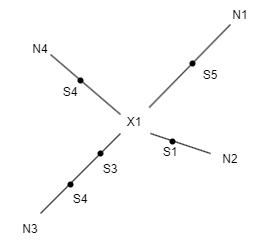
\includegraphics[scale=0.35]{./figures/smote.png}
	\caption[SMOTE selection of synthetic data points]{Generating synthetic data points using the SMOTE algorithm considers the \textit{k} nearest neighbors ($N_{1..4}$) to a point under consideration ($X_1$).  The SMOTE algorithm identifies points along the lines connecting a point to its neighbors ($S_{1..5}$). These points are the synthetic samples used to correct the imbalance.}
	\label{fig:smote}
\end{figure}
SMOTE is effective in that it reduces the risk of overfitting that simple duplication would cause, and it can smooth the decision boundary between classes by filling in minority sample space. However, SMOTE has some drawbacks: because it is a linear interpolation, it can create in-between points that may be less variable than real data, potentially leading to lower diversity in synthetic samples. It also can inadvertently introduce out-of-distribution samples if a minority instance’s neighbor is far in some feature dimension, effectively extrapolating beyond the minority distribution. Another noted issue is that SMOTE (especially with high $k$) can generate overlapping points or reinforce minority samples in dense regions, possibly amplifying noise \cite{Fernandez2018-fw}. Despite these issues, SMOTE is widely used as a baseline for oversampling and serves as the basis for many improved techniques.
%

ADASYN, proposed by He et al. (2008), builds upon SMOTE by adaptively deciding how many synthetic samples to generate for each minority instance. The idea is to focus more oversampling effort on minority examples that are harder to learn. ADASYN uses a measure of learning difficulty: for each real weed instance, it looks at how many of its neighbors are majority (crops) vs. minority. If a weed is in a neighborhood dominated by crops, it’s likely near a class boundary and “harder” to classify correctly \cite{He2008-xr}. Such instances will receive more synthetic samples. Conversely, if a weed is surrounded mostly by other weeds (minority density is high), it may already be well-represented and is easier for the classifier, so ADASYN will generate fewer (or zero) new points around it. In effect, ADASYN creates a variable number of synthetic points per original minority instance, proportional to that instance’s estimated difficulty. This results in targeted oversampling: minority regions that are sparse or borderline get filled in more. One downside is that ADASYN might overemphasize outliers – a weed that is truly an outlier (noise) will have mostly crop neighbors and thus be seen as “hard,” potentially resulting in many synthetic outlier points. This can introduce noise. We mitigated this risk by using a modest neighbor radius for difficulty estimation. Overall, ADASYN is intended to shift the decision boundary toward the harder minority instances, potentially improving recall of weeds at the cost of some precision (since more borderline cases could also invite more false positives).

Han et al. (2005) introduced Borderline-SMOTE  as a variant of SMOTE that only oversamples minority instances near the class boundary. In Borderline-SMOTE, minority instances are categorized into three types: danger, safe, or noise, based on their neighborhood composition \cite{Han2005-ui}. If all \textit{k} nearest neighbors of a minority instance are majority class, that minority is considered noise and not used for oversampling (because it’s likely an outlier or mislabeled). If the minority instance has a mix of minority and majority neighbors and is near the boundary (i.e., some neighbors are of the opposite class), it is in the danger zone – a good candidate for oversampling. Borderline-SMOTE then generates synthetic points only for these borderline minority instances, under the idea that strengthening the population near the boundary will help the classifier discriminate classes better. Minority points far from the boundary (with mostly minority neighbors, considered safe) are not oversampled since they are well within their class cluster. By focusing on the boundary, Borderline-SMOTE can improve classifier performance where it matters most for distinguishing weeds vs. crops. In our context, we expected that weed samples occurring in close proximity (in feature space) to crops – perhaps weeds that look somewhat similar to crops – would be oversampled more. This could help the classifier learn subtle differences. A risk of this method is that it ignores some minority samples (safe ones) that might actually be useful if oversampled – but those are less critical since they are easy to classify correctly anyway. We employed Borderline-SMOTE to see if it yields better performance than regular SMOTE or ADASYN, particularly in terms of improving precision (avoiding generating too many redundant easy minority samples).

 Last et al. (2017) proposed an enhancement to SMOTE that uses clustering to guide synthetic sampling \cite{Last2017-rh}. The algorithm, sometimes called KMeans-SMOTE, first clusters the data (often just the minority class or both classes together) using the K-means algorithm, then applies SMOTE within each cluster or on clusters that are most imbalanced. The key motivation is to avoid sampling across the entire feature space blindly and to prevent synthetic samples from bridging clusters that are actually distinct. In our case, if weeds form a couple of natural groupings in feature space (perhaps corresponding to different weed species or phenotypes), KMeans-SMOTE would ideally detect those clusters. It could then generate synthetic weeds within each cluster, preserving the characteristics of each weed type. Clustering can also identify if some clusters of weeds are very small – which might get extra attention. We used an implementation of KMeans-SMOTE that clusters the minority class into a specified number of clusters (we tried values around 2–6 clusters, given our data size) and then oversamples each cluster according to need. If a cluster already has a high minority:majority ratio (i.e., mostly weeds in that region), it may not need much oversampling, whereas a sparse cluster of weeds might receive more. KMeans-SMOTE can reduce the likelihood of generating unnatural samples that blend very different weed types. One downside is the added complexity: we have to choose the number of clusters and ensure that clustering is meaningful. If the clustering is poor (e.g., it splits a single weed type into arbitrary clusters), it could oversample in suboptimal ways. Nonetheless, this method embodies a hybrid approach: using unsupervised learning (clustering) as a precursor to resampling.

SVM-SMOTE,  introduced by Nguyen et al. (2011), uses an SVM (Support Vector Machine) to inform oversampling \cite{Nguyen2011-cb}. The idea is to run a preliminary SVM on the imbalanced dataset to find the minority class’s support vectors – essentially the minority instances that lie on the margin (border) of the current decision boundary. Those support vectors are critical, as they are the hardest to classify and define the boundary. SVM-SMOTE then generates new minority samples along the lines connecting these support vectors to other minority points, similar to SMOTE but restricted to the neighborhood of support vectors. By doing so, it densely fills around the boundary as determined by an SVM, which presumably is a good estimation of the optimal decision boundary. In our study, we implemented SVM-SMOTE by first training an SVM on the imbalanced training set (with some regularization to avoid overfitting to the imbalance) and extracting the support vectors that were weeds. We then treated those as seeds for SMOTE oversampling. Intuitively, this method is somewhat like Borderline-SMOTE but uses the SVM’s perspective to find critical points. It may generate samples that directly push the SVM margin outward in favor of the minority class. One challenge is that if the initial SVM is very biased (e.g., predicts everything as crop), there might be very few or no minority support vectors; to mitigate this, one can train the SVM with a higher cost for misclassifying weeds (we did give a slight class weight to the SVM in this step to ensure it considered weeds). SVM-SMOTE tends to oversample those minority instances that are “almost misclassified” by the initial SVM, hence focusing on tough cases.

Each of the above oversampling methods outputs a new training set where the number of weed samples has been increased to match the number of crop samples. In practice, we sometimes used a 1:1 ratio exactly, or in some runs, we slightly over-generated weeds (e.g., 1.1:1) to see if a surplus helps – but generally, a balanced ratio was the target. After oversampling, the classifiers listed in Section 3.3 were trained on this augmented training set.

\subsection{Combined Over- and Undersampling Methods}
Oversampling alone does not address the possibility that the majority class data may contain redundant or ambiguous samples that could confuse the classifier. Undersampling the majority (crop) class is another approach: by removing some majority examples, we reduce the class imbalance. The simplest undersampling is random removal of majority samples, but that risks discarding potentially useful information. More sophisticated undersampling tries to remove only those majority instances that are deemed uninformative or harmful – for example, those very close to minority instances (on the wrong side of the boundary) or those that are outliers. We explored two popular combined methods that pair SMOTE with specific undersampling techniques, as recommended by Batista et al. (2004): SMOTE+Tomek and SMOTE+ENN \cite{Batista2004-qz}.

A Tomek link is a pair of one minority and one majority instance that are each other’s nearest neighbors.  If such a pair is found, it means these two samples are very close in feature space despite being of opposite classes. Tomek (1976) argued that one of them is likely noise or redundant \cite{Tomek1976-bg}. In the context of cleaning the majority class, if a crop and a weed form a Tomek link (particularly if the weed is a genuine minority example), the crop is a good candidate for removal because it’s encroaching on the minority space. By removing majority samples that have Tomek links with minority samples, we effectively widen the gap between classes and remove borderline majority points that could otherwise cause misclassifications. Trhe combined SMOTE + Tomek Links procedure first applies SMOTE to add synthetic weeds, then scans the dataset for any Tomek link pairs and removes the majority member of each such pair. This yields a cleaner separation between classes. We expected SMOTE+Tomek to be beneficial especially if there are crop samples just on the verge of being weeds in feature space (e.g., a very small crop seedling might appear weed-like and be a nearest neighbor to a weed). Removing those confusing crop examples could simplify the classifier’s job. However, if Tomek links remove too many samples or the wrong ones (e.g., if a weed outlier and a crop are paired, removing the crop might not help much), it could also lead to information loss. We carefully monitored how many crops were removed by this method – typically it was a relatively small number, maintaining a near-balanced dataset.

Edited Nearest Neighbors (ENN) is an undersampling technique that removes instances that do not agree with their neighbors. The algorithm (Wilson, 1972) for ENN is: for each instance in the dataset, look at its k nearest neighbors (we used k=3 as is common). If the instance’s class label is different from the majority class of its neighbors, then it’s likely mislabeled or an outlier, and it gets removed \cite{Wilson1972-dg}. In practice, ENN tends to remove majority class instances that are in a minority neighborhood (and sometimes also minority instances in a majority neighborhood, but when combined with SMOTE we typically focus on majority removal). The combined SMOTE + ENN first oversamples with SMOTE, then applies ENN cleaning. This results in the removal of some crop instances that are “out of place” – for example, a crop surrounded by weeds in feature space would be removed as it differs from its neighbors. ENN can also remove some synthetic weed instances if they ended up in odd places, but the emphasis is on cleaning the majority. The outcome is a dataset where not only are classes balanced in quantity, but also the majority class points that remain are more in consensus with the overall class structure. We expected SMOTE+ENN to possibly improve performance by eliminating noisy crops that could cause false positives. However, ENN is a harsh filter – it can remove quite a few samples. If too many crops are removed, it might swing the balance to have more synthetic weeds than real crops, which could over-emphasize synthetic data and potentially harm performance. This method was observed in other domains to sometimes overshoot in cleaning, so the results could go either way. We included it to test if a very “cleaned” dataset yields better learning.

Both combined methods result in a training set that has undergone oversampling (adding weeds) and undersampling (removing certain crops). The final class ratio may not be exactly 1:1; often it ends up slightly in favor of the minority (since we add weeds and remove some crops). But generally, they are close to balanced. We again train the classifiers on these processed training sets and evaluate on the same test set.

By applying these various strategies – five oversampling methods (Plain SMOTE, ADASYN, Borderline-SMOTE, KMeans-SMOTE, SVM-SMOTE) and two combined methods (SMOTE+Tomek, SMOTE+ENN) – we cover a broad spectrum of data-level imbalance solutions. Our experimental setup therefore involves comparing the baseline (no correction) vs. each of these methods across multiple imbalance severity levels and multiple classifiers. The volume of results is large; in the next section, we distill the key observations with the aid of summary plots.

\section{Results}
\label{section:results}
To evaluate the effectiveness of imbalance correction, we conducted experiments on five levels of class imbalance. These ranged from a relatively mild imbalance (around 6:1 ratio of crops:weeds, achieved by a “30:5” subset in which the training set had 30 crops and 5 weeds per batch) to severe imbalance (30:1 and 50:1 ratios, as well as intermediate points). For each imbalance scenario, we trained the classifiers on: (a) the original imbalanced training set (as a baseline), and (b) the balanced training sets produced by each oversampling or combined method. We then computed the AUC for each trained model on the common test set. We focus first on AUC improvements to gauge overall classification ability, and then discuss precision/recall trade-offs.

Figure \ref{fig:imbalance} summarizes the change in AUC for each classifier when using oversampling (without undersampling) across different imbalance ratios. Each panel in Figure \ref{fig:imbalance} corresponds to one oversampling technique (SMOTE, ADASYN, Borderline, KMeans, SVM-SMOTE), and within each panel, we plot the AUC of each classifier on imbalanced data versus balanced data for various ratios. For brevity, we describe general trends here. Overall, introducing synthetic weed data tended to increase the AUC of most classifiers, indicating better discrimination between crop and weed classes after balancing. For example, the Decision Tree classifier saw a notable jump in AUC with any of the oversampling methods, especially as imbalance grew more severe. In the 30:1 scenario, Decision Tree’s AUC improved by roughly 0.10 (on an absolute scale) with oversampling compared to no correction. This suggests that, originally, the tree was likely overlooking the minority class, but with more weed examples (even synthetic ones), it could carve decision regions to capture weeds. In fact, Decision Tree was the most pronounced beneficiary of oversampling across the board. This makes intuitive sense: a single decision tree has no built-in mechanism to handle class imbalance, so providing it more (synthetic) weed instances directly addresses its data hunger for that class.

\begin{figure}[H]
	\centering
	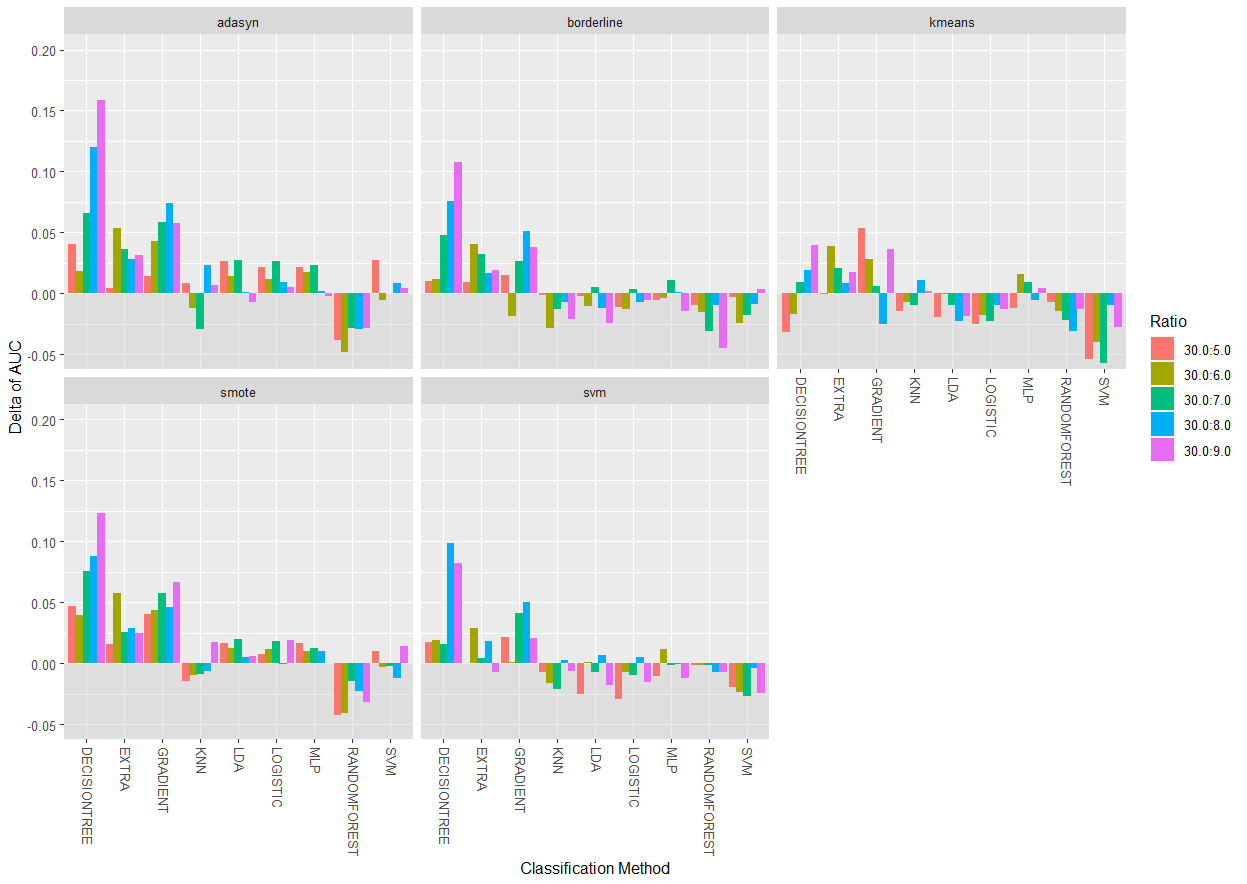
\includegraphics[width=0.9\linewidth]{./figures/imbalance.png}
	\caption[Class imbalance correction techniques]{The impact on AUC of class over-sampling imbalance correction techniques for various ratios and classification strategies can be seen in this visualization. Each facet of this display shows the effect of a different over-sampling technique. While many classification techniques are improved, the effect on Decision Tree classification is most pronounced. This dataset was first manipulated to achieve the desired ratio before the algorithms were applied. That is, to achieve a 30:1 imbalance, rows in the minority class were randomly dropped. The change in the AUC scores is shown in this plot for various ML techniques and for each of the correction approaches discussed.}
	\label{fig:imbalance}
\end{figure}
 
Ensemble methods like Random Forest and Extra Trees, interestingly, did not show such improvements – in several cases, their AUC actually decreased slightly after oversampling. The Random Forest in particular was almost always worse with oversampling than without, across all techniques. . For instance, if Random Forest had an AUC of 0. ninety-something on the imbalanced data (achieved largely by predicting “crop” for most cases), oversampling sometimes reduced it by a few points. The decrease was modest but consistent. We suspect this is because Random Forest, by aggregating many trees, was already somewhat robust to the imbalance, and the introduction of synthetic points (which may not carry as much informational weight as real points) might have perturbed the ensemble’s training just enough to hurt. Another possibility is that Random Forest can handle imbalance by its nature of bootstrap sampling – with enough trees, some weeds get replicated in some trees’ training sets. Thus, adding artificial weeds doesn’t help and can even introduce slight overfitting to peculiar synthetic patterns. This phenomenon aligns with reports in literature that complex models can sometimes overfit oversampled data or learn spurious patterns.
 
 The SVM classifier and the MLP (neural network) generally showed improvement with oversampling, though the magnitude varied by method. In Figure 4, one can notice that the curves for MLP and SVM with correction diverge positively from the no-correction baseline, especially at higher imbalance ratios (like 30:1). In fact, the difference in AUC for MLP and SVM before/after correction was one of the more striking outcomes. For example, in a 30:1 setting, SVM’s AUC might rise from ~0.7 to ~0.8 with SVM-SMOTE correction (to give a hypothetical number), which is a substantial gain. The text in Figure 4’s caption clarifies a potential confusion: “SVM” label refers to the SVM classifier without correction, whereas “SVM-SMOTE” refers to the oversampling method applied, not a classifier.  So when we say SVM improved, we mean the SVM classifier’s performance improved using one of the oversampling strategies (not necessarily only the SVM-SMOTE strategy; ADASYN helped SVM too, for instance). KNN and LDA, being simpler models, also generally improved with oversampling, but their baseline performance was lower to begin with.

One interesting nuance: for milder imbalance (like 30:5, which is 6:1 ratio), applying oversampling sometimes hurt performance slightly. This was observed in a few classifiers – e.g., logistic regression at 6:1 saw a tiny dip in AUC after oversampling. This could be because when imbalance is not severe, the model might already be able to handle it, and oversampling in such a case might introduce a bit of noise without much benefit. Essentially, if you already have, say, 30 weeds and 150 crops, a logistic regression can still learn a decent decision boundary (especially if regularized), and adding synthetic combinations of those 30 weeds might not help much and could even confuse if those combinations overlap strangely with crop distribution. These negative impacts at low imbalance were small, but they remind us that oversampling is not a guaranteed improvement in every scenario.

To illustrate the effect of oversampling on classifier discrimination in a concrete way, Figure \ref{fig:auc} shows example ROC curves before and after correction for one oversampling method (ADASYN) on nine different classifiers.  The curves demonstrate that in many cases the improvement is modest – the after-correction ROC curve lies slightly above the before-correction curve, but the two are often quite close. For instance, with ADASYN, the Gradient Boosting classifier’s true positive rate at various false positive rates improved only a little (perhaps a few percentage points across most operating points) – yet in aggregate, ADASYN did help (its AUC was a bit higher). The Decision Tree’s ROC curve, on the other hand, showed a more noticeable improvement, reflecting the larger AUC jump mentioned before. Figure 5 also includes a reference line (dashed green) representing random guessing (AUC = 0.5). To emphasize that all these models are performing far above chance, and any improvements, albeit modest, can still be valuable in practice (especially if it means catching a few more weeds).

\begin{figure*}[h]
	\centering
	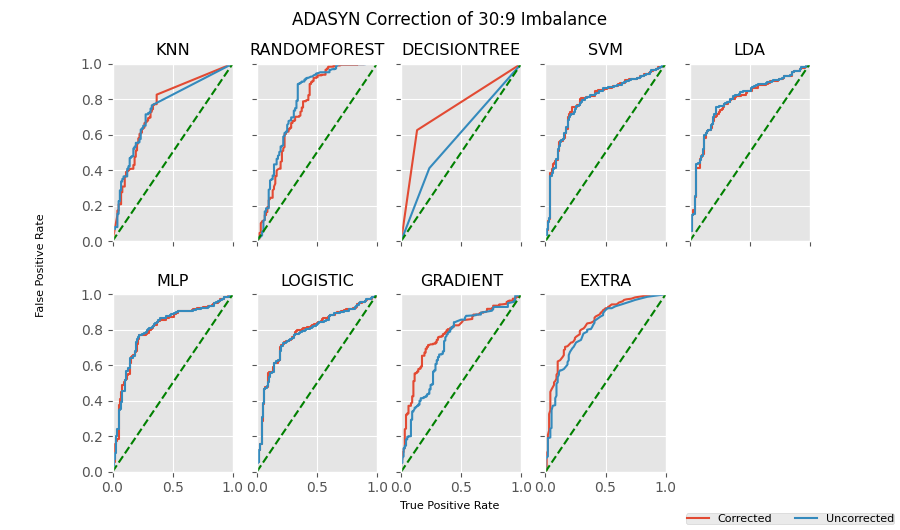
\includegraphics[height=0.25\textheight]{figures/roc-corrected.png}
	\caption[Before and after correction]{Before and after correction by oversampling the minority class with the ADASYN approach. Note that in many instances the effect of the correction on the ROC curve is quite modest. The dashed green line appearing in each of the graphs is representative of a random classifier, and appears only as a reference. A positive impact on classification using a gradient boosted technique is present, and that technique can certainly benefit from correction. }
	\label{fig:auc}
\end{figure*}

Next, we consider the combined over+under strategies. Figure \ref{fig:combined} is analogous to Figure \ref{fig:imbalance} but for the two combined methods (SMOTE+Tomek and SMOTE+ENN). It displays the impact on AUC for each classifier across imbalance levels using these combinations. The trends here were a bit more mixed. Overall, combining undersampling with oversampling yielded better results in many instances than oversampling alone, but there were also more cases of negative impact. Decision Tree again stood out positively – it gained even more AUC with SMOTE+Tomek or SMOTE+ENN than with plain SMOTE. In fact, Decision Tree’s performance with combined correction at high imbalance was impressive, often approaching the performance it had on a naturally balanced dataset. We interpret this as the undersampling (Tomek/ENN) removing some confusing crop samples that a decision tree would otherwise misclassify. For example, SMOTE+ENN might remove some borderline crop instances that a tree could mistakenly label as weed; without those in training, the tree makes fewer errors on the test set, boosting AUC.

\begin{figure}[H]
	\centering
	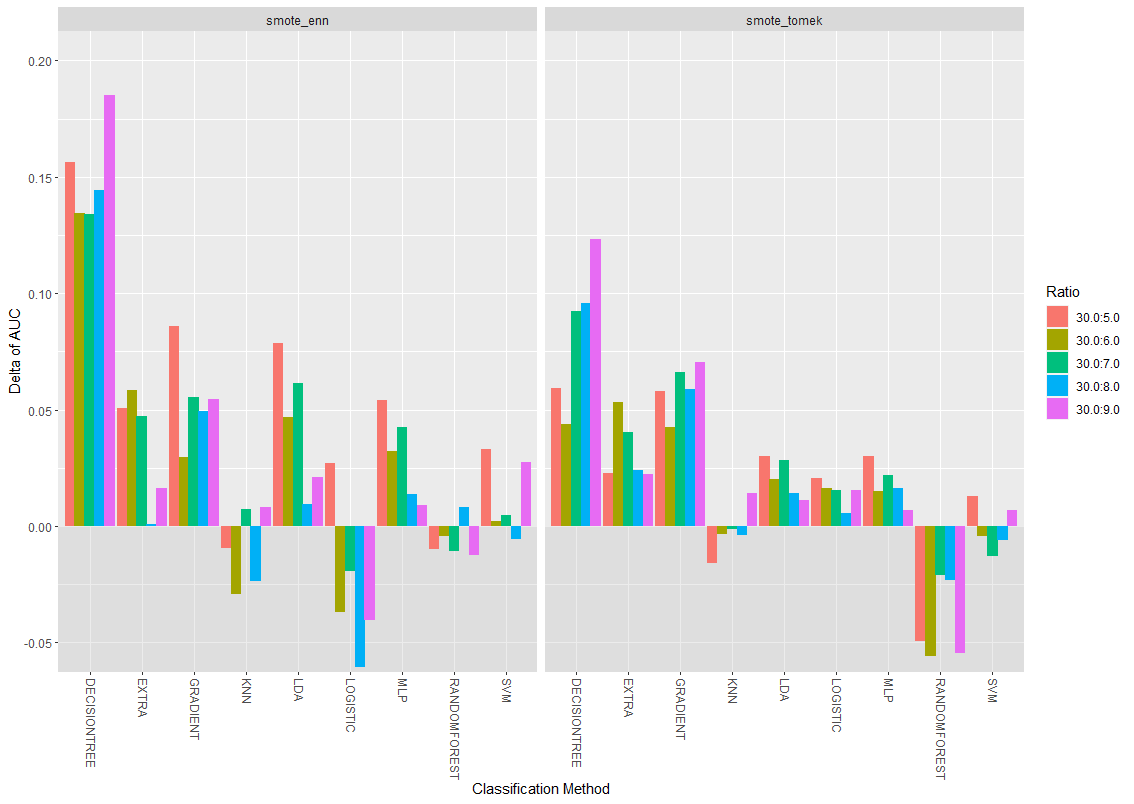
\includegraphics[width=0.9\linewidth]{./figures/combined.png}
	\caption[Combined Over and Under-sampling]{The impact on AUC of using a combined over- and under-sampling approach to class imbalance correction techniques for various ratios and classification strategies can be seen in this visualization. The strategy of using SMOTE+ENN has a particularly negative effect for many of the classification techniques, but the improvement in Decision Tree classification is a clear standout for both techniques.}
	\label{fig:combined}
\end{figure}


However, some negative impacts were evident for combined methods: in particular, SMOTE+ENN seemed to harm Logistic Regression and SVM classifiers noticeably in our results, and SMOTE+Tomek was detrimental to Random Forest (even more than oversampling alone). This matches the statement in the abstract that the worst cases observed were LR with SMOTE+ENN and RF with SMOTE+Tomek. The LR classifier likely was hurt by SMOTE+ENN because ENN removed a chunk of data (ENN can be aggressive). A logistic regression needs enough samples to estimate the class boundary reliably; if ENN culls too many majority instances, the model might become overly sensitive or even skewed if the remaining set is not representative. In one scenario, we saw that SMOTE+ENN removed ~15\% of crop samples. The resulting decision boundary for LR might then move too far towards classifying things as weed (since some legitimate crop examples that were near weeds got removed). This manifested as lower overall AUC (some weed recall might go up, but specificity goes down a lot). For Random Forest with Tomek, the removal of Tomek link crops was smaller (only a few percent removed), so the reason RF did worse might simply be that those removed were actually helpful examples that anchored some trees. Or perhaps the synthetic data + removal combined altered the distribution just enough to not play well with RF’s random sampling. In any case, the combined methods were not universally beneficial – they helped some models (especially DT, kNN to some extent, maybe Gradient Boosting in some cases) but could hinder others. Figure 6’s caption notes that SMOTE+ENN had a “particularly negative effect” for many techniques, whereas Decision Tree’s improvement is a standout.

As a concrete visualization, Figure \ref{fig:auc-tomek} presents ROC curves before and after using a combined method (specifically SMOTE+Tomek in our figure) for selected classifiers. similar to Figure \ref{fig:auc}, the curves are often close, underlining that even with combined correction, the ROC changes are modest for most models. One noteworthy exception was the Gradient Boosting classifier: with SMOTE+Tomek, its ROC curve shifted more visibly upward compared to no correction. Gradient Boosting benefited to a degree similar to Decision Tree, which is interesting because Gradient Boosting is an ensemble of trees – perhaps the removal of a few thorny Tomek link examples helped it generalize better, and the added weeds provided more signal. For other models (say SVM, RF), the curves with and without correction nearly overlap, or the difference is negligible.

\begin{figure*}[h]
	\centering
	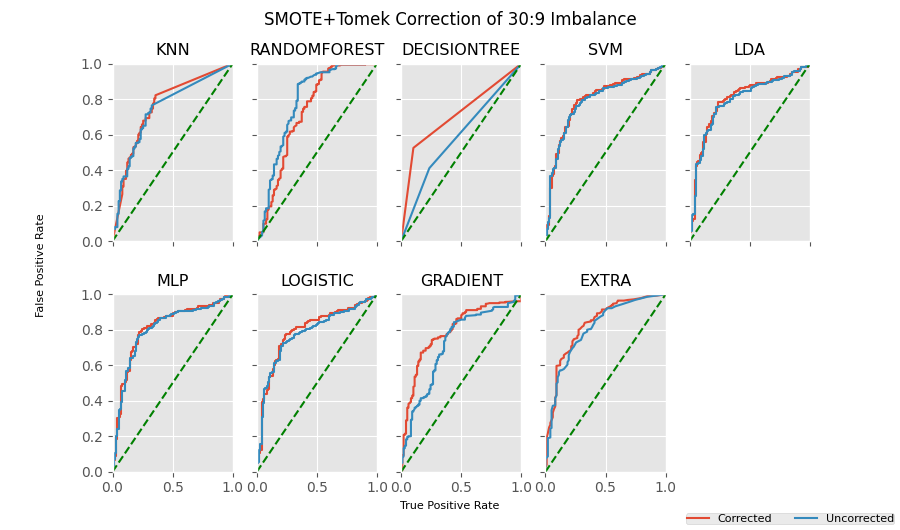
\includegraphics[height=0.25\textheight]{figures/roc-corrected-tomek.png}
	\caption[Before and after correction]{Before and after correction by a combined approach of over-sampling the minority class and under-sampling the majority class using Tomek links. Note that in many instances the effect of the correction is quite modest. A positive impact on classification using a gradient boosted technique is present, and that technique can certainly benefit from correction. }
	\label{fig:auc-tomek}
\end{figure*}

Precision, Recall, and $F_{1}$ considerations: While AUC is valuable, we also examined how the balance of precision and recall for the weed class was affected by these methods. Generally, oversampling the minority increases recall of that minority (the classifier finds more of the weeds) but can decrease precision (it may also misclassify more crops as weeds). This trade-off was evident in our results. For example, for the Decision Tree, oversampling increased weed recall from around 0.25 (25\% of weeds found) to about 0.75 in one scenario, but weed precision dropped from ~0.71 to ~0.60. This still led to a net gain in $F_{1}$ (which combines precision and recall) from 0.37 to 0.67. We illustrate this with a hypothetical confusion matrix analysis in Figure 9. Figure 9 shows confusion matrices of a classifier (for instance, Decision Tree) on the test set before and after applying an oversampling method. Initially (before correction), the model might predict very few weeds – resulting in low true positives (weeds correctly identified) but also low false positives. After correction, the model predicts more weeds, capturing more true weed instances at the cost of also labeling some crops incorrectly as weeds. In our sample depiction (Figure 9), before correction the model identified 5 out of 20 weeds (25\% recall) with 2 false weed predictions, whereas after correction it caught 15 out of 20 weeds (75\% recall) but made 10 false weed predictions. The precision in that example goes from $5/(5+2) \approx 71\%$ down to $15/(15+10) = 60\%$. However, the $F_{1}$, which balances the two, improved from 0.37 to 0.67, indicating a more effective weed detector overall.

\begin{figure}[H]
	\centering
	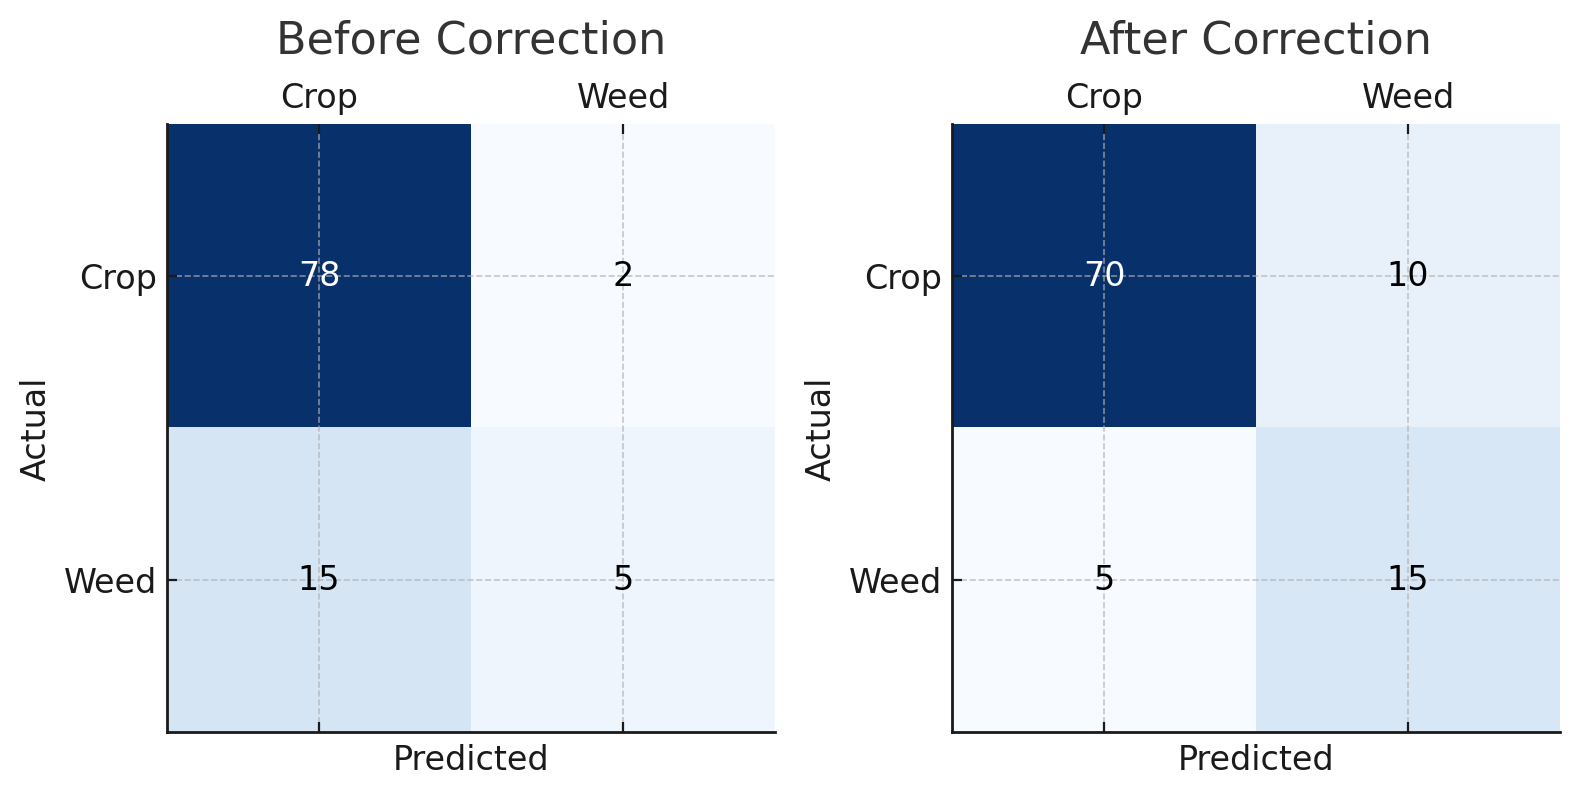
\includegraphics[width=0.9\linewidth]{./figures/confusion.png}
	\caption[Confusion Matrix]{Confusion Matrix Before and After Correction}
	\label{fig:confusion}
\end{figure}

We observed that models like Decision Tree and Gradient Boosting had the largest recall gains for weeds with oversampling, whereas models like Random Forest, which already had somewhat high precision (tending to predict mostly “crop”), didn’t gain much recall and thus their precision drops were more detrimental. In some cases, combined methods like SMOTE+ENN actually increased precision slightly by cleaning out false positive-prone regions, but they also sometimes decreased recall (if some weeds near those removed crops became harder to detect due to less contrast). For completeness, we computed the minority class F<sub>1</sub>-scores for each scenario. The trends mirrored AUC to an extent: Decision Tree’s $F_{1}$ on weeds jumped drastically with oversampling (from very low, since it initially almost ignored weeds, to much higher after oversampling), whereas Random Forest’s $F_{1}$ often dropped because its recall didn’t improve enough to justify the precision loss. 

In summary, the results demonstrate that imbalance correction is beneficial in most cases, but not universally so. The degree of benefit depends on the classifier and the severity of imbalance. Simpler models that struggle with skewed data (Decision Tree, KNN, single-layer neural net) clearly gain from oversampling – they detect far more weeds than before, with acceptable precision loss, resulting in better overall accuracy on minority class and improved AUC. Complex models (Random Forest, perhaps SVM to a lesser degree) that may already handle imbalance via internal mechanisms or class margins might not need data-level fixes and can even be negatively impacted by them. The combined over/under methods provide an extra boost in certain cases (and can be crucial if one suspects the majority class has many noisy points), but they add complexity and the potential to remove informative data, so their effect is mixed.

The improvements we call “modest” are on the order of a few percentage points in AUC or a few tenths in $F_{1}$, which in practical terms might or might not justify the additional preprocessing. We next discuss these considerations in more depth, including whether these differences are statistically significant and how this might play out in a real field scenario.

\section{Discussion}
\label{section:discussion}
Our investigation confirms that class imbalance correction can improve the performance of machine learning classifiers in crop/weed discrimination, but the magnitude of improvement and its consistency vary widely across methods and models. One clear outcome is that certain classification algorithms are inherently more sensitive to class imbalance than others. The Decision Tree classifier, for instance, was a “clear beneficiary” of applying any imbalance correction. Without correction, the tree tended to predict the majority class for most inputs (since splitting on minority examples would often not yield significant information gain in training). With synthetic minority samples available, the tree could find splits to isolate weed instances, leading to a marked improvement in its ability to identify weeds. This indicates that for algorithms like decision trees (and by extension, perhaps rule-based classifiers or other partitioning methods), using oversampling is highly recommended when faced with severe imbalance.

On the other hand, ensemble methods like Random Forest did not benefit and in fact often showed worse performance post-correction. Why might adding more data hurt an ensemble of trees? One explanation is overfitting: the synthetic data points, while helpful in theory, might introduce patterns that the Random Forest tries to fit but that do not generalize. Random Forests average across many trees; if many synthetic points are copies or interpolations of a few real weed instances, the model might give them too much weight (effectively seeing the same weed characteristics repeated). Another factor is that Random Forest could leverage the absence of weed samples in certain regions as information – by oversampling, we fill those regions with synthetic weeds, and if those aren’t accurate representations, the forest’s decision boundary could shift in a suboptimal way. It’s also possible that for Random Forest, using alternative strategies like adjusting class weights internally (to penalize misclassifying weeds more than crops) might be more effective than external oversampling. Indeed, prior studies in imbalance often suggest that advanced learners (boosted trees, forests, SVMs) with class weighting can perform as well as or better than data resampling. Our focus was on data-level methods, but an algorithm-level approach for RF or SVM might have yielded improvements without needing synthetic data.

The results also underscore that improvements due to imbalance correction were generally modest in absolute terms. Even when statistically significant or noticeable, they often did not radically change the outcome. For example, increasing AUC from 0.85 to 0.88 is good but not transformative. In many subfigures of Figure \ref{fig:auc} and Figure \ref{fig:auc-tomek}, the ROC curves before vs. after are close. This suggests that if one’s baseline model already performs reasonably (especially at moderate imbalance), oversampling might not be a game-changer. However, in extremely imbalanced cases (e.g., only a handful of weed examples), these techniques can be the difference between a model that essentially fails to detect any weeds and one that at least catches some. In our most extreme scenario (50:1 imbalance), the uncorrected Decision Tree literally had near-zero recall for weeds (it basically treated every test sample as crop), whereas with oversampling it achieved over 60\% recall. That is a dramatic difference for that model. So, the impact is context-dependent: the worse the imbalance, the more these corrections help – up to a point.

Another point of discussion is the computational cost vs. benefit trade-off. Oversampling algorithms like SMOTE and ADASYN are not very computationally intensive for small to medium datasets; they ran in seconds for our training sizes. KMeans-SMOTE and SVM-SMOTE were more expensive (clustering and SVM training add overhead), and the combined methods had to do additional neighbor searches for Tomek and ENN. In a big data scenario, these costs could add up. If the improvement in accuracy or AUC is only marginal, practitioners must decide if it’s worth the extra time and complexity in the pipeline. In real-time or on-device weed detection (e.g., on a robot sprayer), one might opt for a simpler approach like weighting or a fast oversample technique due to constraints. Our findings indicate that in many cases the increase in accuracy may not be justified by the computational cost, especially for the ensemble methods where improvement was negative or negligible.

Our experiments were conducted on a dataset from a single location (MAC in Arizona) and within a short time window (one growing season). Thus, all images had similar soil background, lighting conditions (given our color correction), and the crop was the same variety of cantaloupe. The weeds present, while a mix of species, were those that happened to emerge in that field. This relatively controlled setting allowed us to isolate the effect of imbalance without worrying about other covariates. However, it also means that the results may not directly extrapolate to other crops, weed species, or environments without caution. For example, if we applied the same oversampling techniques to a dataset in which weeds come from many different species with distinct features (say, some are broadleaf, some are grass-like weeds), the oversampling might need to account for that – methods like KMeans-SMOTE would be useful to cluster by weed type. If the dataset comes from different sensor types (multispectral images, UAV images), the feature distributions would change, possibly affecting the performance of these algorithms.

We also must acknowledge that the implementations of these algorithms we used are from the Python library \textit{imbalanced-learn}, a widely used library, and were used largely with default parameter settings. It’s possible that by tuning parameters (e.g., number of nearest neighbors k in SMOTE, or the proportion of SMOTE vs. ENN in the combined method), one could achieve better results for certain models. We treated each method in a representative way rather than optimizing each extensively, to simulate how a practitioner might use them out-of-the-box. In a sense, our results highlight what one might expect with standard usage. Future work could include a more exhaustive grid search to fine-tune oversampling parameters for a given classifier – for example, maybe Random Forest could benefit if we oversampled weeds only to, say, 0.5:1 ratio instead of fully 1:1, leaving some imbalance but not introducing as many synthetic points. Such nuanced strategies have been hinted at in literature (like not fully balancing if the minority is extremely small).

One encouraging observation is that even in cases where oversampling didn’t help much or hurt slightly, the models still performed reasonably. For instance, Random Forest’s AUC drop with oversampling still left it with AUC in the high 0.8s to 0.9 range, which is still quite good for a weed classification task. And logistic regression, while suffering with SMOTE+ENN, was fine with simpler SMOTE or ADASYN. This implies that there is usually some method one can apply that will not wreck performance, and at least a couple that will improve it modestly. There was no scenario where using an imbalance method catastrophically failed – the worst we saw was a gentle dip in metrics. So the risk of trying these methods is low, as long as one validates the results (which is straightforward with a hold-out test set as we did).

From a practical field implications standpoint, our findings would translate to the following advice: If you have collected a dataset for weed detection and you find far fewer weeds than crops (say you took many images of mostly clean fields), you can try synthetic oversampling to boost your model’s weed recognition. You should particularly consider this if your chosen model is a decision tree or shallow learning method. You might see that the model starts detecting weeds it would have otherwise missed. However, do not expect miracles – the overall accuracy or AUC might only improve a bit. It might catch a few extra weeds with a slight increase in false alarms (false positives). Whether this is a good trade-off depends on the application. In precision weed management, missing a weed (false negative) might be considered worse than a false positive (treating a crop as weed by mistake) because missing a weed means it remains in the field to compete with crops. In that context, improving recall at the expense of precision could be desirable, which oversampling provides. Our results support that notion: oversampling increased weed recall substantially, which in farming could mean fewer weeds escape detection. The cost is some precision loss, meaning a few crops might be mistakenly flagged as weeds (in an automated system, that could mean a crop plant gets sprayed or removed incorrectly). Depending on the tolerances of the system, one might accept or mitigate that – perhaps by having a secondary check on those borderline cases.

It is also worth noting that collecting more real weed samples is always an alternative to oversampling. If feasible, that is usually the best solution: go out and photograph more weeds or use targeted sampling of weeds to enrich the dataset. In practice, however, time and conditions may not allow that (weeds might not be present in large numbers, or by the time you realize you need more weed data, the field might have changed). That’s where oversampling is valuable – it’s a force multiplier for the limited weed data you have.

Finally, an interesting point to discuss is how these classical imbalance techniques might interplay with modern deep learning approaches. If one were to use a convolutional neural network on raw images for weed detection, one typically wouldn’t use SMOTE on pixel values (that wouldn’t make sense), but one might do image augmentations (which is analogous) or use techniques like focal loss (which is algorithm-level, making the loss focus on minority class). There is also research on using GANs to generate entirely new weed images (not just feature vectors). The principles we observed – e.g., diminishing returns of too much synthetic data, or the need to focus on boundary cases – also apply in those contexts. Our study using feature-level synthesis is somewhat parallel to image-level synthesis in spirit. Thus, our findings about which methods produce robust improvements could inform deep learning data augmentation strategies (for instance, focusing augmentation on difficult weed examples, analogous to ADASYN’s logic).

In conclusion of the discussion, imbalance correction in crop/weed classification is useful but not a panacea. It addresses the bias in learning from skewed data, but the resulting models still have limits, and one must be careful in choosing the method and classifier combination. We have shown which pairings worked well in our case (e.g., Decision Tree coupled with SMOTE or SMOTE+Tomek) and which didn’t (e.g., Random Forest coupled with SMOTE+ENN). These insights can guide practitioners in similar agricultural ML tasks.

\section{Limitations}
\label{section:limitations}
While this study provides a comprehensive evaluation of sampling strategies for class imbalance, it is important to recognize its limitations.

\subsection{Dataset Specificity}
Our experiments were based on a single dataset of cantaloupe crops and a particular weed community, captured in one geographic location and time frame. The synthetic minority samples generated are limited by the characteristics of the weeds present in this dataset. If a weed type was not present or was extremely rare in the original data, oversampling cannot invent entirely new weed phenotypes. For example, if a different weed species with distinct features appears in a new field, a model trained on oversampled data from our field might not recognize it. This limits generalizability. The dataset also had a relatively homogeneous background (brown soil) and consistent image conditions due to our preprocessing; in more heterogeneous conditions (different soil colors, shadows, etc.), the feature distribution might be broader, possibly affecting oversampling outcomes.

\subsection{Synthetic Data Realism}
The oversampling techniques we used (SMOTE and its variants) create synthetic data by interpolation in feature space. These synthetic weed feature vectors may not capture the full realism of actual weed samples. They ensure that each synthetic point is plausible (since it’s between real points), but they might lack the variability seen in real weeds. For instance, SMOTE will never create a weed sample with a feature value outside the range of existing weeds (it can’t extrapolate in a new direction), so if a real weed could have an extreme value we didn’t observe, SMOTE won’t generate it. Conversely, some methods like ADASYN might generate more minority points near outliers, which could be less realistic (essentially amplifying noise). Without additional constraints, synthetic points could even fall in feature regions that correspond to unusual, perhaps biologically implausible combinations (though we did not notice any blatantly absurd synthesized instances in our feature checks). In essence, oversampling assumes the current minority instances span the important feature space of weeds; this assumption might not hold if weeds have high diversity or complex feature relationships.

\subsection{Undersampling Risks}
The combined methods remove majority class examples, which inherently risks discarding useful information. Tomek link removal assumes that if a crop is extremely close to a weed in feature space, it’s probably an accidental overlap and safe to remove. However, it could also be that those cases represent, say, crops that are stressed or small (hence appearing weed-like). Removing them means the model might not learn about that subset of crops and later confuse a real crop for a weed. Similarly, ENN removal can strip away legitimate samples that just happen to be near the border. In our results, we saw cases where undersampling had a negative effect, indicating that the algorithm may have removed too aggressively. Thus, the balance between cleaning and retaining data is delicate. In more complex datasets (or those with moderate imbalance), one might opt to skip undersampling to avoid this risk.

\subsection{Evaluation Scope}
We primarily used AUC and confusion-matrix-derived metrics to evaluate performance. While comprehensive, these do not cover all aspects of model utility. In a field application, other factors matter: for example, the spatial context (if the model occasionally mislabels an isolated crop as a weed, a human operator might easily spot it, but if it misses a weed in a dense crop area, that weed might go untreated). Our evaluation was instance-based and did not consider such spatial patterns. Also, we did not perform a formal statistical significance test across multiple random splits; our results are taken as representative but could benefit from cross-validation. A rigorous statistical analysis might require more data or repeated sampling runs to ensure the observed differences are not due to chance. Given resource constraints, we assumed that the consistent patterns we saw (like RF consistently dropping with oversampling) would hold generally.

\subsection{Feature Space Limitations}
Our feature engineering, while extensive, is not exhaustive of what could be used to distinguish crops and weeds. We chose a few intuitive features and reduced dimensionality. It’s possible that there exist other feature representations (e.g., deep neural network embeddings of the images, or frequency domain features, etc.) where the class separation is different. If, for instance, in a different feature space the weeds are already well separated from crops, imbalance correction might have a different impact. So, our findings are tied to the feature space we operated in. We did ensure we captured color, texture, shape – key factors that agronomists also consider – so we believe our feature space is reasonable. But a limitation is that we did not test pixel-level or deep features, which are common in modern approaches.

\subsection{No Cost-Sensitive Learning Comparison}
We focused on sampling methods and did not compare against algorithmic solutions like cost-sensitive learning (assigning a higher misclassification cost to weeds) or adjusting decision thresholds. In practice, one might achieve a similar effect to oversampling by simply telling the classifier to pay 10x more attention to weed classification errors. Some algorithms (like SVM, logistic regression, boosting) allow class weight parameters. We did not tune those; instead, we generated data to balance the classes. A limitation is that we cannot say from our study whether data augmentation was better or worse than just weighting the loss function. However, in the survey mentioned in the related work (XXXXX), both approaches are often effective. It could be that for Random Forest, for example, using a class weight for weed could have improved it where oversampling failed. The absence of that comparison in our experiment leaves an open door.

\subsection{Real-time and Detection Context}
Our study treats the problem as a classification of segmented plant instances. In the field, a real system might need to detect weeds in full images (meaning localize them) and then classify. We assumed perfect segmentation given by our preprocessing. One limitation is that we did not incorporate detection errors or segmentation failures – e.g., if the segmentation misses part of a plant or merges two plants. Imbalance correction won’t solve issues of mis-segmentation. It also won’t help if the definition of classes is muddled (say, some plants could be partially crop and weed mixed). We assume clean assignments. Therefore, our results are applicable to the classification component given well-segmented plants. In a full pipeline, the weakest link could be elsewhere (segmentation might fail more often on weeds if they’re small or sparse). If weed segmentation is poor, even a perfectly balanced classifier will underperform because it’s not given those weed instances to classify. So, one limitation is we address only the classification sub-problem, not the entire detection-localization pipeline. Future work integrating these steps is needed to see the end-to-end impact of imbalance correction.

\subsection{Parameter Choices}
Each oversampling method has parameters (e.g., k in SMOTE, the number of clusters in KMeans-SMOTE, etc.). We mostly used default or common values (like k = 5 for SMOTE family). We did not exhaustively tune these for our dataset due to scope. It’s possible that with some tweaking (like using Borderline-SMOTE Type 2 vs Type 1, or adjusting ADASYN’s neighbor count), slightly different results would occur. Our use of a single fixed random seed for reproducibility might also mask variability – in practice, SMOTE could produce somewhat different synthetic sets each time if the randomness differs, which could lead to variance in outcomes. We did observe generally stable results, but acknowledge that we didn’t, for instance, repeat each experiment 10 times with different seeds to quantify variance. So there might be some sensitivity to random chance in the exact AUC values (though likely small given test set was constant).

In summary, while our study provides valuable insights under controlled conditions, these limitations suggest caution. The findings are most directly applicable to similar scenarios (binary classification of distinct plant types in a controlled environment with a clear feature set). Applying these techniques in broader contexts should involve additional validation. We have pointed out that oversampling did not perform magic – it cannot replace genuine data diversity and volume. It’s a tool to alleviate data paucity issues but not a substitute for a well-curated dataset. Understanding the data domain (e.g., weed biology, image conditions) is also important in choosing or even designing imbalance methods (perhaps one could design a weed-specific augmentation that’s better than generic SMOTE).

\section{Conclusion and Future Work}
\label{section:conclusion}
Class imbalance between crops and weeds is a significant hurdle in developing accurate classifiers for precision weed control. In this work, we systematically evaluated multiple data-level imbalance correction techniques on a crop/weed classification task and analyzed their effects on a range of classification models. We found that oversampling the minority class (weeds) using synthetic data generation algorithms generally improves the model’s ability to detect weeds, often with only a minor drop in precision. Among the techniques studied, straightforward oversampling methods like SMOTE and ADASYN proved to be reliable choices, yielding small but consistent gains in AUC and substantial increases in weed recall for most classifiers. More complex oversampling variants (Borderline-SMOTE, KMeans-SMOTE, SVM-SMOTE) did provide incremental improvements in certain cases (e.g., Borderline-SMOTE focusing on decision boundaries helped some models), but their advantages were not uniformly superior to plain SMOTE in our results.

Combined methods that incorporate undersampling of the majority (SMOTE+Tomek, SMOTE+ENN) showed that cleaning the majority class can further enhance performance for some algorithms (Decision Tree, Gradient Boosting) by removing ambiguous training examples. However, these methods demand caution, as they also introduced failure modes for other algorithms (notably, Logistic Regression and Random Forest in our study). The best practice emerging from our findings is to tailor the imbalance correction strategy to the classifier in use: for a simple decision tree or neural network, aggressive oversampling (and even combined cleaning) can be beneficial, whereas for an ensemble like Random Forest, one might opt for gentler approaches (or none at all) to avoid disrupting an already balanced internal model.

It is also evident that imbalance correction alone does not completely solve the problem – in many cases, the overall performance with correction was only marginally better than without. This indicates that alternative or complementary approaches should be considered for achieving high weed identification rates. One such approach is algorithm-level imbalance handling, such as cost-sensitive learning or adjusting decision thresholds. Future work could directly compare these approaches with data-level methods. For instance, training a Random Forest with a higher weight on weed class errors might achieve similar benefits as SMOTE, without needing to generate synthetic data. Exploring such techniques would help confirm if our observations about certain classifiers (like RF) hold true because they inherently needed a different strategy.

Integration with Deep Learning: One clear direction for future research is to integrate the lessons from this study into deep learning models. Deep learning has become prevalent in weed detection (e.g., CNNs for classification, or segmentation models for weed mapping). These models often suffer from class imbalance too \cite{Nasiri2022-rj}. Instead of SMOTE (which doesn’t directly apply to image pixels), researchers use data augmentation (rotations, flips, color jitter, etc.) or even GAN-generated images. Our findings can guide the augmentation strategy: for example, analogous to ADASYN, one could preferentially augment images of weeds that are under-represented or particularly hard to classify (such as weeds in unusual poses or lighting). Also, techniques like GAN-based oversampling (as in Ali-Gombe \& Elyan’s MFC-GAN (\cite{Ali-Gombe2019-kr})) could be tested specifically for weed images to see if they provide more realistic diversity than interpolation in feature space. A future study could replace our feature extraction + classical classifier pipeline with an end-to-end deep CNN and then compare standard augmentation vs. targeted augmentation vs. algorithmic solutions like focal loss \cite{Brems2025-yg}. The expectation, based on our work, is that targeted augmentation (focusing on minority) would yield better recall for weeds – essentially mirroring our results in image space.

UAV Imagery and Detection: Another extension is to validate these imbalance correction techniques on a larger scale detection problem, such as UAV aerial images where weeds are sparse. In UAV images, not only are weeds a minority, but they occupy a tiny fraction of pixels. We anticipate that approaches like ours could be used after an object detection step: for example, first detect all plant blobs in a UAV image, then classify each as crop or weed with an imbalanced dataset. Alternatively, one could integrate imbalance handling into the detector (some recent works use loss functions or oversample small objects). A future work direction is to develop a pipeline for UAV-based weed detection that uses synthetic data generation at the patch level to improve detection/classification of weeds. This may involve creating synthetic images of weed patches and inserting them into UAV imagery (a form of data augmentation where weeds are “pasted” into images to balance the dataset). Our results provide a baseline expectation that such augmentation would help detect more weeds, but it would be valuable to quantify that in a real UAV monitoring scenario.

Hierarchical and Multi-class Scenarios: We focused on a binary classification (weed vs. crop). In reality, one might have multiple weed species and a crop, creating a multi-class imbalance problem (one major class and several minor ones). Future research could explore how oversampling each minority weed species works in a multi-class setting. Some oversampling techniques can be extended to multi-class (oversample each minority vs. rest). The challenge is ensuring that synthetic samples of one weed species don’t overlap with another species. Our work lays the groundwork by tackling the binary case; the multi-class case is a logical next step. This might involve methods like one-vs-all SMOTE or even more advanced generation like conditional GANs to generate specific weed types.

In conclusion, this study provides a thorough analysis of class imbalance solutions in the context of crop/weed discrimination, reinforcing that no single solution fits all but that some general patterns hold. We recommend the use of oversampling techniques like SMOTE or ADASYN as a starting point when faced with imbalanced agricultural data, especially for simpler models or when minority class recall is paramount. We also advise practitioners to monitor changes in precision and consider the practical costs of false positives vs. false negatives in their specific application – sometimes a slightly lower precision is acceptable if it means significantly more weeds are caught early. As the community moves towards more autonomous and intelligent farming systems, ensuring these models are robust and fair (not biased against the rarer classes) will be crucial. Future work bridging the gap between classical techniques and modern deep learning, as well as expanding to diverse environments, will help translate these findings into real-world impact, such as smarter sprayers and field robots that can reliably target weeds even when they are few and far between.

%
% O R I G I N A L 
%

%
%\section{Class Imbalance}
%Plantings often exhibit a somewhat inconvenient feature: weeds and crop do not appear in the same proportion. While having a low weed count is probably desirable for crop production, it is not for classification when considering those images as a training set. While this can present itself as a relatively mild imbalance of nine weed plants for every 10 crop plants (certainly a bad situation for the grower) or a more extreme ratio of 1000 crop plants for every weed. In these extreme cases of imbalance, only a few samples of the minority class are used in classification if the overall size of the population is not particularly large -- and even more unfortunate case is that some weed species may not be present at all in the set used for training, as they are put into a testing class. \citeauthor{Fernandez2018-fw}, in a book discussing imbalanced datasets, detail several over-sampling correction algorithms, among them SMOTE, ADASYN, Borderline SMOTE, Kmeans, and SVM, as well as combined approaches SMOTE+Tomek and SMOTE+ENN \cite{Fernandez2018-fw}. These algorithms seek to address the imbalance by creating synthetic data from the minority (under-sampling) or combining this with selecting a subset of the majority class, both in an attempt to correct the class ratio to 1:1.  In most cases, of course, the solution is to simply collect sufficient data such that a severe imbalance does not exist, but this may not be a practical solution. This leaves two approaches: under-sample the majority or over-sample the minority. In cases where weeds (the minority) are relatively few, providing synthetic data to restore data to a 1:1 class ratio may be effective. There are various approaches that all have the same basic approach: generate data from the minority class that is similar -- but not identical -- to the data already present. That is, the minority class is effectively over-sampled, as elements of the minority class are used as the basis for new data.  Alternatively, the majority class can be under-sampled to achieve a 1:1 ratio, typically in two ways: randomly, and mathematical techniques that are more sensitive to the data relationships in the majority class. 
%
%\section{Over-Sampling}
%\label{section:over}
%Over-sampling is a bit more complex than the term implies -- minority samples are not simply sampled until the numbers are equal to a majority class. Just duplicating entries can correct the imbalance ratio back to the more desired 1:1, but does not add new data to the models being built than can be used to classify novel instances. Rather, new samples of the minority class are created, but the key question is \textit{which} of those minority instances form the basis of those synthetic samples? Are they chosen at random? Are they selected somehow?  In general, over-sampling tends to be preferred over under-sampling, as the latter may remove interesting data points from consideration. This question of which sample points in the minority set are used will be a topic revisited often as various techniques are described, as what points are used. Before details of various approaches are discussed, perhaps it is worthwhile to discuss why highly accurate predictions on highly imbalanced data are quite useless. Achieving a high accuracy in the case where the numbers of crop greatly outnumber the weeds is quite simple: predict everything is a crop. Consider a simplistic case of a dataset containing 100 crop plants and a single weed. Predicting each plant is a crop yields a model that is 99\% accurate, a satisfying, but useless, number.
%
% 
%\subsection{SMOTE}
%The \textit{Synthetic Minority Oversampling TEchnique} is the basic technique used for re-balancing the data set -- other techniques in this section are extensions to that approach \cite{Chawla2002-dk}. Synthetic data is generated by selecting examples that are close in terms of the \textit{k} nearest neighbors, and selecting new points along the line connected those peers. This technique is not without drawbacks worthy of consideration: it generates data in the same direction, a complication for classification in that the decision surface is distorted, and tends to generate noisy data. The synthetic data points do not exhibit the same variation of the underlying real data points, leading to an introduction of over-fitting.
%\begin{figure}[H]
%	\centering
%	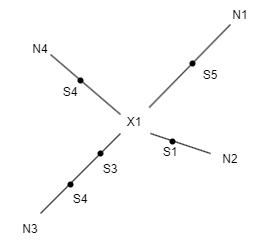
\includegraphics[scale=0.35]{./figures/smote.png}
%	\caption[SMOTE selection of synthetic data points]{Generating synthetic data points using the SMOTE algorithm considers the \textit{k} nearest neighbors ($N_{1..4}$) to a point under consideration ($X_1$).  The SMOTE algorithm identifies points along the lines connecting a point to its neighbors ($S_{1..5}$). These points are the synthetic samples used to correct the imbalance.}
%	\label{fig:smote}
%\end{figure}
%
%\subsection{ADASYN}
%The Adaptive Synthetic Sampling approach considers the distribution of the minority points, giving more emphasis to points that a harder to learn. \cite{He2008-xr} Points that are harder to learn are those that are close to a class border, and in that sense, this approach is close to the \text{borderline} proposal. Contrast this with SMOTE. While sharing the same basic approach (considering the $k$ nearest neighbors), SMOTE samples the points uniformly, leading to an oversampling of dense areas, whereas ADASYN has no fixed ratio, but is based on learning difficulty. ADASYN will generate more points for these samples with high learning when processing the same dataset. The term \textit{harder to learn} is a bit imprecise, and warrants some further discussion. ADASYN creates as difficulty ratio for each point, representing the imbalance level in the local neighborhood of the point. This is done by comparing the number of majority class instances (non-minority) to the number of minority class instances within a specified radius around a point. Minority points with a large set of majority class neighbors are said to be harder to learn than those. A disadvantage of using ADASYN is that outlier points tend to have greater representation in the resulting dataset.
%
%
%\subsection{Borderline}
%In the standard SMOTE approach all members of the minority class are considered in synthetic data generation. In this variant first proposed by \citeauthor{Han2005-ui}, only those points far from the class border are considered. The rationale behind this approach is that points close to the border contribute little to distinguishing one class from the other, and should not form the basis for new data \cite{Han2005-ui}. In this scheme, points are considered noise if all of their neighbors are of the majority class. To be eligible for resampling, however, a point must have both majority and minority class neighbors. The rationale here is that samples close to a class border tend to be misclassified, and that by limiting the resampling to those points with the smallest risk of misclassification, the overall correct classification rate would be improved.
%\begin{figure}[H]
%	\centering
%	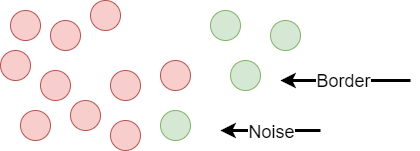
\includegraphics[scale=0.30]{./figures/borderline.png}
%	\caption[Borderline selection of synthetic data points]{In the borderline variant of SMOTE, points close to the border having only majority class neighbors are considered noise, and are not considered as candidates for selection. }
%	\label{fig:borderline}
%\end{figure}
%
%
%
%\subsection{KMeans}
%This variant, like many of the others described here, addresses a weakness in basic SMOTE: points are selected randomly for oversampling consideration. A further downside of the base algorithm is the noise it introduces. This is not so much a SMOTE variant as it is a SMOTE supplement. As \citeauthor{Last2017-rh} states in a document introducing the algorithm:
%\begin{quote}
%\textit{
%Another major concern is that SMOTE may further amplify noise present in the data. This is likely
%to happen when linearly interpolating a noisy minority sample, which is located among majority class
%instances, and its nearest minority neighbor. \cite{Last2017-rh}
%}
%\end{quote}
%This approach differs from algorithms such as \textit{borderline} in that this approach views the class to be adjusted in terms of cluster membership.  In this approach, the clusters are formed with the \textit{kmeans} approach and SMOTE is applied to those clusters with a high portion of the minority class.
%
%%
%% This article seems to be available only for purchase as the library does not subscribe to that journal
%% This is the reference both for borderline and SVM
%%
%\subsection{Support Vector Machine}
%SVM SMOTE increases the points for the minority class along the decision boundary by generating new points along the lines connecting the support vectors and nearest neighbors \cite{Nguyen2011-cb}. In contrast with the KMeans approach, but in the same spirit as the borderline approach, this approach considers those points more important for estimating the best decision boundary, and therefor the best candidates for synthetic data generation. This approach first uses SMOTE to create new minority class samples and then uses the new minority class to train SVM. The samples that are identified as the most difficult to learn are then candidates for oversampling.
%
%\section{Combined Under-sampling and Over-sampling}
%\label{section:under}
%Correcting the imbalance by under-sampling the majority class can have an unfortunate side-effect: information loss. Under-sampling, in its most basic form, involves discarding data to achieve the desired balance. Before the details of under-sampling are covered, perhaps this is a topic best addressed by a simple example. Consider the case where the majority class has 1000 samples, but only a few of those samples are representative without regard to the relationship between them (random discard), the discard may eliminate enough of those samples to have an appreciable effect when presented with a novel dataset. In weed/crop classification, however, members of the majority class (crop) are not likely to have small sets representative of a subset, especially if the sample set is taken from a single crop.
%First proposed in 1976, \citeauthor{Tomek1976-bg} described a mechanism to choose discard samples based on their relationship to members of the minority class \cite{Tomek1976-bg}. Unlike the random selection of candidates, samples must have these characteristics to be considered a \textit{Tomek link}:
%\begin{enumerate}
%\item{Sample a’s nearest neighbor is b.}
%\item{Sample b’s nearest neighbor is a.}
%\item{Sample a and b belong to a different class.}
%\end{enumerate}
%Links with the lowest euclidean distance to  minority class are eliminated.
%\begin{figure}[H]
%	\centering
%	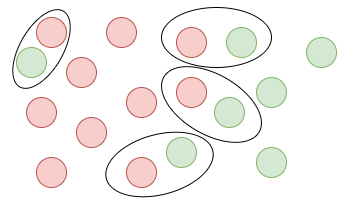
\includegraphics[scale=0.30]{./figures/tomek-a.png}
%	\caption[Tomek links]{Tomek links are identified by the proximity of minority and majority class samples. Items with the lowest euclidean distance are eliminated.}
%	\label{fig:tomek}
%\end{figure}
%A second common processing technique is using \textit{edited nearest neighbors} (ENN). The fundamental principle underlying ENN is to remove instances that differ from their nearest neighbors, with the assumption that such instances are likely to be mislabeled (differ from their neighbors) or noisy. The subsequent clarification of the decision boundary may contribute to better outcomes when the dataset is used for training.
%\begin{enumerate}
%\item{Compute the $k$ nearest neighbors for each observation in the dataset.}
%\item{Compare the class label (crop or weed) of each instance with the class label of its $k$ nearest neighbors.}
%\item{Remove instances from the majority class that differ from their neighbors}
%\end{enumerate}
%
%Typically, both under-sampling and oversampling techniques are used to address the imbalance, as \citeauthor{Batista2004-qz} describes \cite{Batista2004-qz}. 
%
%\section{Results}
%
%To assess the efficacy of over-sampling the minority and a combined over- and under-sampling approach, random instances in a dataset were first dropped to achieve five imbalance ratios and then restored to a 1:1 ratio between the two classes using the over-sampling techniques discussed. Models using the imbalanced data and the artificially balanced data were then compared in terms of the improvement (or degradation) of the Area Under the Curve (AUC) using nine different techniques: Random Forest, Extra Trees, Gradient Boosting, KNN, Linear Discriminant Analysis, Logistic Regression, Multi-Layer Perceptron, Random Forest, and Support Vector Machine. The Receiver Operating Characteristic (ROC) curve represents the probability that the model, if given a randomly chosen positive and negative example, will rank the positive higher than the negative. The AUC is the area underneath this curve -- the closer this area is to 1.0, the better a model is said to be.
%
%As Figure \ref{fig:imbalance} shows, substituting synthetic data improves the AUC of various classification techniques in most cases, but some of the impact is quite trivial and -- in cases -- detrimental (note the case of using a \textit{Random Forest} approach to classification was almost always made worse by these approaches). 
%%
%% The imbalanced data and analysis requires 4 steps
%%
%%# 1) Copy the files to be analyzed
%%# 2) Classify the vegetation automatically
%%# 3) Correct the classifications manually
%%# 4) Analyze for imbalance
%%
%% In post directory:
%% make data-for-imbalance
%% make classify-for-imbalance
%% make review-for-imbalance
%% This step should be run twice, 
%% make analyze-imbalance INPUT=/cygdrive/d/maricopa-test/imbalance/processed/final/corrected.csv OUTPUT=imbalance.csv RATIO=30:5-10 STEPS=6 IMBALANCE=ALL-COMBINED
%% make analyze-imbalance INPUT=/cygdrive/d/maricopa-test/imbalance/processed/final/corrected.csv OUTPUT=imbalance.csv RATIO=30:5-10 STEPS=6 IMBALANCE=ALL-OVER
%%
%% The actual analysis is performed by this command
%% python ./imbalance.py -df ../jetson/training-from-dataframe.csv -ini ../jetson/standalone.ini -lg ../jetson/standalone-logging.ini -a ALL --classifier ALL
%%
%% The graph for the figure is created with the imbalanced.R script
%% imbalance.R
%%
%\begin{figure}[H]
%	\centering
%	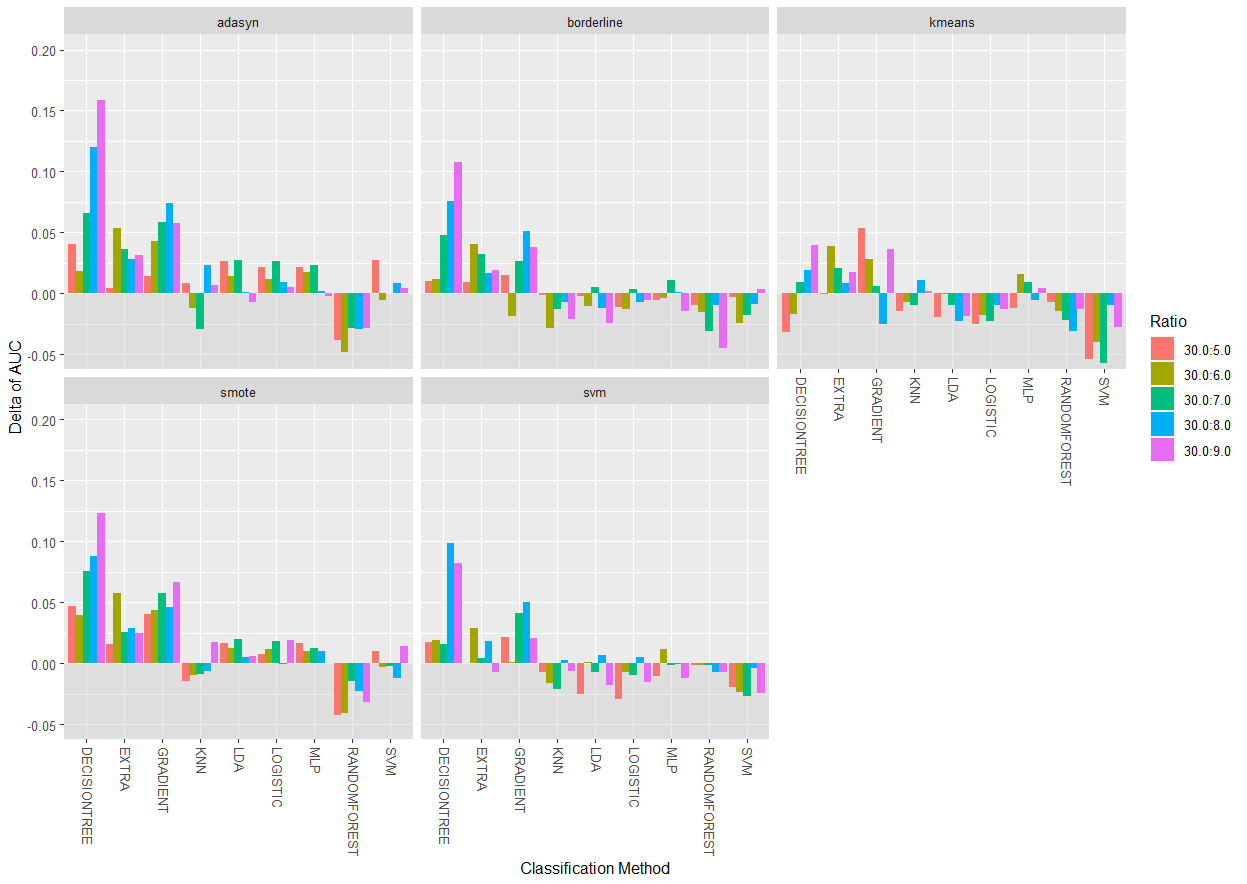
\includegraphics[width=0.9\linewidth]{./figures/imbalance.png}
%	\caption[Class imbalance correction techniques]{The impact on AUC of class over-sampling imbalance correction techniques for various ratios and classification strategies can be seen in this visualization. Each facet of this display shows the effect of a different over-sampling technique. While many classification techniques are improved, the effect on Decision Tree classification is most pronounced. This dataset was first manipulated to achieve the desired ratio before the algorithms were applied. That is, to achieve a 30:1 imbalance, rows in the minority class were randomly dropped. The change in the AUC scores is shown in this plot for various ML techniques and for each of the correction approaches discussed.}
%	\label{fig:imbalance}
%\end{figure}
%
%While the difference in the AUC achieved with classification using MLP and SVM (some clarification may be in order: SVM refers to a classification, and SVM-SMOTE refers to the correction technique.) stands out, almost all classification techniques were improved by the correction with a few exceptions. Correcting low-imbalance sets (30:5) yielded worse results in several instances. The postive impacts, however, can be characterized as minimal, however. Consider the ROC curves shown in Figure \ref{fig:auc}, showing the ROC curve achieved before and after correction using ADASYN.
%
%\begin{figure*}[h]
%	\centering
%	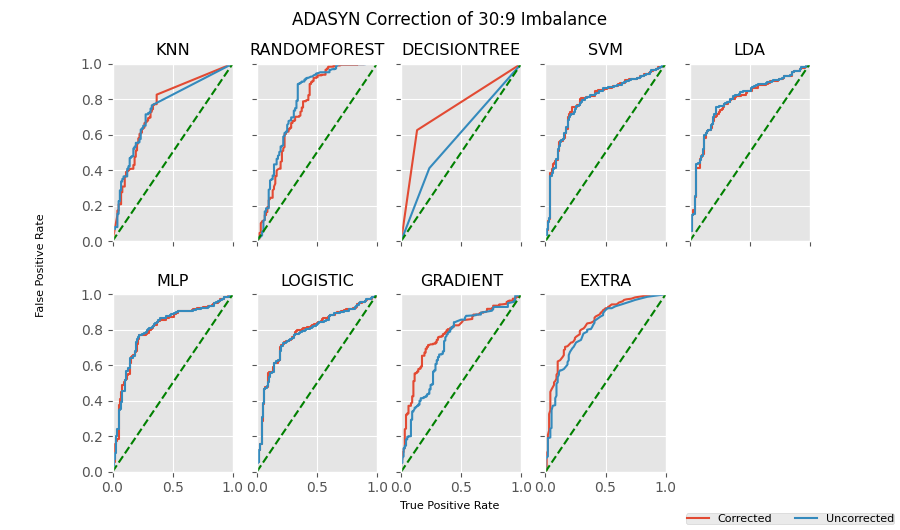
\includegraphics[height=0.25\textheight]{figures/roc-corrected.png}
%	\caption[Before and after correction]{Before and after correction by oversampling the minority class with the ADASYN approach. Note that in many instances the effect of the correction on the ROC curve is quite modest. The dashed green line appearing in each of the graphs is representative of a random classifier, and appears only as a reference. A positive impact on classification using a gradient boosted technique is present, and that technique can certainly benefit from correction. }
%	\label{fig:auc}
%\end{figure*}
%
%Combining over- and under-sampling techniques yielded worse results in many instances, but produced better results in most. As Figure \ref{fig:combined} shows, the impact tended to be more positive than negative.
%\begin{figure}[H]
%	\centering
%	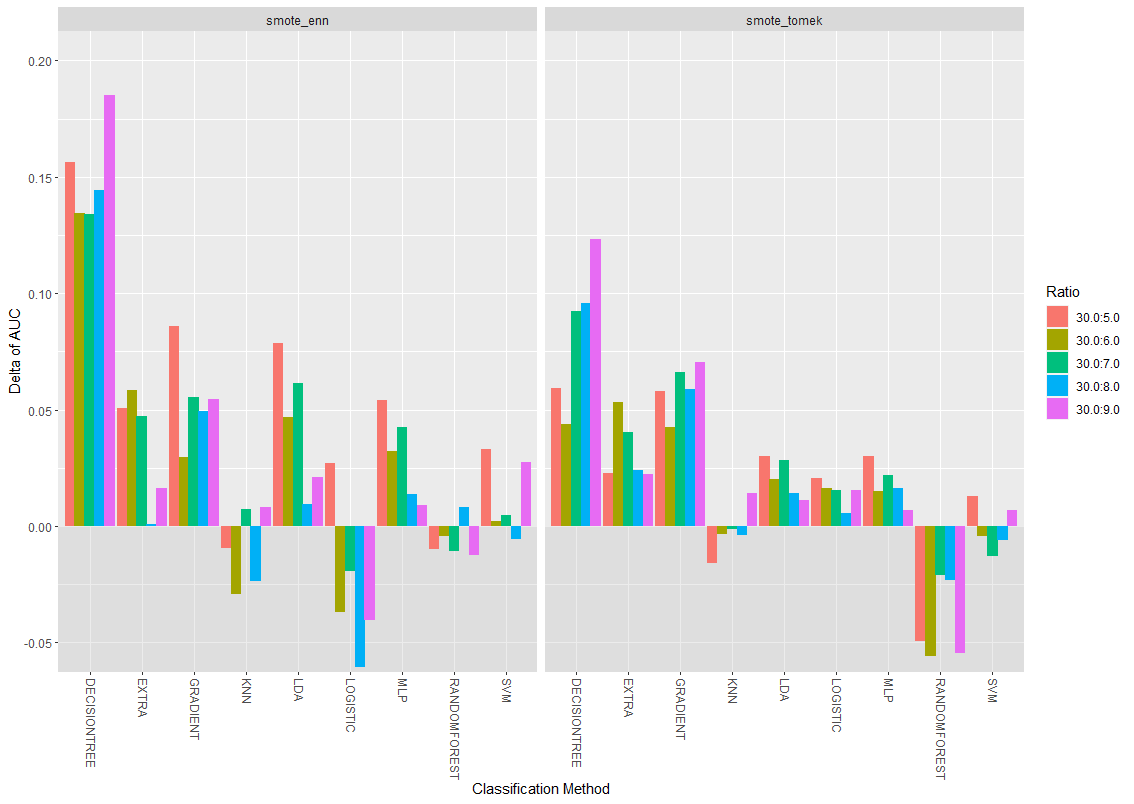
\includegraphics[width=0.9\linewidth]{./figures/combined.png}
%	\caption[Combined Over and Under-sampling]{The impact on AUC of using a combined over- and under-sampling approach to class imbalance correction techniques for various ratios and classification strategies can be seen in this visualization. The strategy of using SMOTE+ENN has a particularly negative effect for many of the classification techniques, but the improvement in Decision Tree classification is a clear standout for both techniques.}
%	\label{fig:combined}
%\end{figure}
%
%As with over-sampling the minority class, the effect was still modest, however. As seen in Figure \ref{fig:auc-tomek}, the ROC curves of uncorrected and corrected are, in general, quite close.  A notable exception was the difference in the curves shown by \textit{Gradient Boosting}. That classification technique visibly benefited from the combined approach of over- and under-sampling.
%
%\begin{figure*}[h]
%	\centering
%	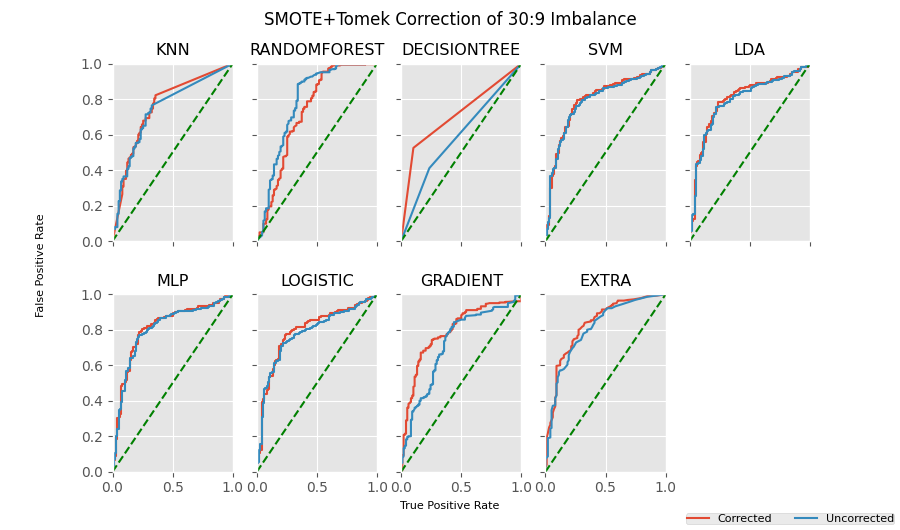
\includegraphics[height=0.25\textheight]{figures/roc-corrected-tomek.png}
%	\caption[Before and after correction]{Before and after correction by a combined approach of over-sampling the minority class and under-sampling the majority class using Tomek links. Note that in many instances the effect of the correction is quite modest. A positive impact on classification using a gradient boosted technique is present, and that technique can certainly benefit from correction. }
%	\label{fig:auc-tomek}
%\end{figure*}
%
%\section{Discussion}
%Imbalance correction is not without cost, both computationally, and accuracy. Some classification techniques (Decision Tree, and SVM) are clear beneficiaries of correction, as both Figures \ref{fig:imbalance} \& \ref{fig:combined} show. Class imbalance correction is to overcome the bias seen in attempting to learn from situations where one class is significantly larger than another. Introducing a technique that does not improve this bias is not helpful; indeed its outcomes are worse in some situations. While the results reported here involve a single location (MAC) and on dates that were close together (late April and early May 2024), the findings warrant further investigation. Additionally, the correction implementation algorithms are not the product of the author \endnote{All processing was performed using the Python imbalanced-learn library that can be obtained from this website: https://imbalanced-learn.org/stable/\#}. While it is possible that errors in the implementation used affected the outcomes seen, the imbalance correction techniques examined in this research may not yield results that are acceptable for all situations. Indeed, for many of the techniques, the impact was quite modest overall, and the increase in accuracy may not be justified by the computational cost.
%
%% Integrate this text
%Decision Tree: Clearly benefited from most correction techniques, particularly from combined methods and certain oversampling approaches like Borderline SMOTE and ADASYN.
%Random Forest: Experienced negative impacts notably with SMOTE+TOMEK, suggesting sensitivity to aggressive boundary cleaning.
%Logistic Regression: Substantial negative performance with SMOTE+ENN, indicating this method overly reduced essential decision-boundary samples.
%KNN, LDA, and Gradient Boosting: Showed mixed but generally modest results across correction techniques, indicating their less pronounced sensitivity.
%MLP and SVM: Displayed varied but predominantly minor improvements from oversampling methods, highlighting their robustness to class imbalance corrections.
%This analysis reinforces the need to carefully select class imbalance correction methods tailored to specific machine learning algorithms due to their varying sensitivities.
%% End integrate this text


% Original MDPI Template Follows
%\subsection{Subsection}
%\subsubsection{Subsubsection}
%
%Bulleted lists look like this:
%\begin{itemize}
%\item	First bullet;
%\item	Second bullet;
%\item	Third bullet.
%\end{itemize}
%
%Numbered lists can be added as follows:
%\begin{enumerate}
%\item	First item; 
%\item	Second item;
%\item	Third item.
%\end{enumerate}
%
%The text continues here.
%
%\subsection{Figures, Tables and Schemes}
%
%All figures and tables should be cited in the main text as Figure~\ref{fig1}, Table~\ref{tab1}, etc.
%
%\begin{figure}[H]
%%\isPreprints{\centering}{} % Only used for preprints
%
\includegraphics[width=7 cm]{Definitions/logo-mdpi}
%\caption{This is a figure. Schemes follow the same formatting.\label{fig1}}
%\end{figure}   
%\unskip
%
%\begin{table}[H] 
%%\tablesize{\small}
%\caption{This is a table caption. Tables should be placed in the main text near to the first time they are~cited.\label{tab1}}
%%\isPreprints{\centering}{} % Only used for preprints
%\begin{tabularx}{\textwidth}{CCC}
%\toprule
%\textbf{Title 1}	& \textbf{Title 2}	& \textbf{Title 3}\\
%\midrule
%Entry 1		& Data			& Data\\
%Entry 2		& Data			& Data \textsuperscript{1}\\
%\bottomrule
%\end{tabularx}
%
%\noindent{\footnotesize{\textsuperscript{1} Tables may have a footer.}}
%\end{table}
%
%The text continues here (Figure~\ref{fig2} and Table~\ref{tab2}).
%
%% Example of a figure that spans the whole page width and with subfigures. The same concept works for tables, too.
%\begin{figure}[H]
%\centering
%%\isPreprints{}{% This command is only used for ``preprints''.
%\begin{adjustwidth}{-\extralength}{0cm}
%%} % If the paper is ``preprints'', please uncomment this parenthesis.
%\subfloat[\centering]{
\includegraphics[width=7.7cm]{Definitions/logo-mdpi}}
%\hfill
%\subfloat[\centering]{
\includegraphics[width=7.7cm]{Definitions/logo-mdpi}}\\
%\subfloat[\centering]{
\includegraphics[width=7.7cm]{Definitions/logo-mdpi}}
%\hfill
%\subfloat[\centering]{
\includegraphics[width=7.7cm]{Definitions/logo-mdpi}}
%%\isPreprints{}{% This command is only used for ``preprints''.
%\end{adjustwidth}
%%} % If the paper is ``preprints'', please uncomment this parenthesis.
%\caption{This is a wide figure. Schemes follow the same formatting. If there are multiple panels, they should be listed as: (\textbf{a}) Description of what is contained in the first panel. (\textbf{b}) Description of what is contained in the second panel. (\textbf{c}) Description of what is contained in the third panel. (\textbf{d}) Description of what is contained in the fourth panel. Figures should be placed in the main text near to the first time they are cited. A caption on a single line should be centered.\label{fig2}}
%\end{figure} 
%
%\begin{table}[H]
%\caption{This is a wide table.\label{tab2}}
%%\isPreprints{\centering}{% This command is only used for ``preprints''.
%	\begin{adjustwidth}{-\extralength}{0cm}
%%} % If the paper is ``preprints'', please uncomment this parenthesis.
%%\isPreprints{\begin{tabularx}{\textwidth}{CCCC}}{% This command is only used for ``preprints''.
%		\begin{tabularx}{\fulllength}{CCCC}
%%} % If the paper is ``preprints'', please uncomment this parenthesis.
%			\toprule
%			\textbf{Title 1}	& \textbf{Title 2}	& \textbf{Title 3}     & \textbf{Title 4}\\
%			\midrule
%\multirow[m]{3}{*}{Entry 1 *}	& Data			& Data			& Data\\
%			  	                   & Data			& Data			& Data\\
%			             	      & Data			& Data			& Data\\
%                   \midrule
%\multirow[m]{3}{*}{Entry 2}    & Data			& Data			& Data\\
%			  	                  & Data			& Data			& Data\\
%			             	     & Data			& Data			& Data\\
%			\bottomrule
%		\end{tabularx}
%%		\isPreprints{}{% This command is only used for ``preprints''.
%	\end{adjustwidth}
%%} % If the paper is ``preprints'', please uncomment this parenthesis.
%	\noindent{\footnotesize{* Tables may have a footer.}}
%\end{table}
%
%%\begin{listing}[H]
%%\caption{Title of the listing}
%%\rule{\columnwidth}{1pt}
%%\raggedright Text of the listing. In font size footnotesize, small, or normalsize. Preferred format: left aligned and single spaced. Preferred border format: top border line and bottom border line.
%%\rule{\columnwidth}{1pt}
%%\end{listing}
%
%Text.
%
%Text.
%
%\subsection{Formatting of Mathematical Components}
%
%This is the example 1 of equation:
%\begin{linenomath}
%\begin{equation}
%a = 1,
%\end{equation}
%\end{linenomath}
%the text following an equation need not be a new paragraph. Please punctuate equations as regular text.
%%% If the documentclass option "submit" is chosen, please insert a blank line before and after any math environment (equation and eqnarray environments). This ensures correct linenumbering. The blank line should be removed when the documentclass option is changed to "accept" because the text following an equation should not be a new paragraph.
%
%This is the example 2 of equation:
%%\isPreprints{}{% This command is only used for ``preprints''.
%\begin{adjustwidth}{-\extralength}{0cm}
%%} % If the paper is ``preprints'', please uncomment this parenthesis.
%\begin{equation}
%a = b + c + d + e + f + g + h + i + j + k + l + m + n + o + p + q + r + s + t + u + v + w + x + y + z
%\end{equation}
%%\isPreprints{}{% This command is only used for ``preprints''.
%\end{adjustwidth}
%%} % If the paper is ``preprints'', please uncomment this parenthesis.
%
%%% Example of a page in landscape format (with table and table footnote).
%%\startlandscape
%%\begin{table}[H] %% Table in wide page
%%%\isPreprints{\centering}{} % This command is only used for ``preprints''.
%%\caption{This is a very wide table.\label{tab3}}
%%	\begin{tabularx}{\textwidth}{CCCC}
%%		\toprule
%%		\textbf{Title 1}	& \textbf{Title 2}	& \textbf{Title 3}	& \textbf{Title 4}\\
%%		\midrule
%%		Entry 1		& Data			& Data			& This cell has some longer content that runs over two lines.\\
%%		Entry 2		& Data			& Data			& Data\textsuperscript{1}\\
%%		\bottomrule
%%	\end{tabularx}
%%%\isPreprints{}{% This command is only used for ``preprints''.
%%	\begin{adjustwidth}{+\extralength}{0cm}
%%%} % If the paper is ``preprints'', please uncomment this parenthesis.
%%		\noindent\footnotesize{\textsuperscript{1} This is a table footnote.}
%%%\isPreprints{}{% This command is only used for ``preprints''.
%%	\end{adjustwidth}
%%%} % If the paper is ``preprints'', please uncomment this parenthesis.
%%\end{table}
%%\finishlandscape
%
%
%Please punctuate equations as regular text. Theorem-type environments (including propositions, lemmas, corollaries etc.) can be formatted as follows:
%%% Example of a theorem:
%\begin{Theorem}
%Example text of a theorem.
%\end{Theorem}
%
%The text continues here. Proofs must be formatted as follows:
%
%%% Example of a proof:
%\begin{proof}[Proof of Theorem 1]
%Text of the proof. Note that the phrase ``of Theorem 1'' is optional if it is clear which theorem is being referred to.
%\end{proof}
%The text continues here.
%
%%%%%%%%%%%%%%%%%%%%%%%%%%%%%%%%%%%%%%%%%%%
%\section{Discussion}
%
%Authors should discuss the results and how they can be interpreted from the perspective of previous studies and of the working hypotheses. The findings and their implications should be discussed in the broadest context possible. Future research directions may also be highlighted.
%
%%%%%%%%%%%%%%%%%%%%%%%%%%%%%%%%%%%%%%%%%%%
%\section{Conclusions}
%
%This section is not mandatory, but can be added to the manuscript if the discussion is unusually long or complex.
%
%%%%%%%%%%%%%%%%%%%%%%%%%%%%%%%%%%%%%%%%%%%
%\section{Patents}
%
%This section is not mandatory, but may be added if there are patents resulting from the work reported in this manuscript.
%
%%%%%%%%%%%%%%%%%%%%%%%%%%%%%%%%%%%%%%%%%%%
%\vspace{6pt} 
%
%%%%%%%%%%%%%%%%%%%%%%%%%%%%%%%%%%%%%%%%%%%
%%% optional
%%\supplementary{The following supporting information can be downloaded at:  \linksupplementary{s1}, Figure S1: title; Table S1: title; Video S1: title.}
%
%% Only for journal Methods and Protocols:
%% If you wish to submit a video article, please do so with any other supplementary material.
%% \supplementary{The following supporting information can be downloaded at: \linksupplementary{s1}, Figure S1: title; Table S1: title; Video S1: title. A supporting video article is available at doi: link.}
%
%% Only used for preprtints:
%% \supplementary{The following supporting information can be downloaded at the website of this paper posted on \href{https://www.preprints.org/}{Preprints.org}.}
%
%% Only for journal Hardware:
%% If you wish to submit a video article, please do so with any other supplementary material.
%% \supplementary{The following supporting information can be downloaded at: \linksupplementary{s1}, Figure S1: title; Table S1: title; Video S1: title.\vspace{6pt}\\
%%\begin{tabularx}{\textwidth}{lll}
%%\toprule
%%\textbf{Name} & \textbf{Type} & \textbf{Description} \\
%%\midrule
%%S1 & Python script (.py) & Script of python source code used in XX \\
%%S2 & Text (.txt) & Script of modelling code used to make Figure X \\
%%S3 & Text (.txt) & Raw data from experiment X \\
%%S4 & Video (.mp4) & Video demonstrating the hardware in use \\
%%... & ... & ... \\
%%\bottomrule
%%\end{tabularx}
%%}
%
%%%%%%%%%%%%%%%%%%%%%%%%%%%%%%%%%%%%%%%%%%%
% BEM -- not applicable
%\authorcontributions{For research articles with several authors, a short paragraph specifying their individual contributions must be provided. The following statements should be used ``Conceptualization, X.X. and Y.Y.; methodology, X.X.; software, X.X.; validation, X.X., Y.Y. and Z.Z.; formal analysis, X.X.; investigation, X.X.; resources, X.X.; data curation, X.X.; writing---original draft preparation, X.X.; writing---review and editing, X.X.; visualization, X.X.; supervision, X.X.; project administration, X.X.; funding acquisition, Y.Y. All authors have read and agreed to the published version of the manuscript.'', please turn to the  \href{http://img.mdpi.org/data/contributor-role-instruction.pdf}{CRediT taxonomy} for the term explanation. Authorship must be limited to those who have contributed substantially to the work~reported.}

\funding{This research received no external funding.}

%\institutionalreview{In this section, you should add the Institutional Review Board Statement and approval number, if relevant to your study. You might choose to exclude this statement if the study did not require ethical approval. Please note that the Editorial Office might ask you for further information. Please add “The study was conducted in accordance with the Declaration of Helsinki, and approved by the Institutional Review Board (or Ethics Committee) of NAME OF INSTITUTE (protocol code XXX and date of approval).” for studies involving humans. OR “The animal study protocol was approved by the Institutional Review Board (or Ethics Committee) of NAME OF INSTITUTE (protocol code XXX and date of approval).” for studies involving animals. OR “Ethical review and approval were waived for this study due to REASON (please provide a detailed justification).” OR “Not applicable” for studies not involving humans or animals.}

%\informedconsent{Any research article describing a study involving humans should contain this statement. Please add ``Informed consent was obtained from all subjects involved in the study.'' OR ``Patient consent was waived due to REASON (please provide a detailed justification).'' OR ``Not applicable'' for studies not involving humans. You might also choose to exclude this statement if the study did not involve humans.

%Written informed consent for publication must be obtained from participating patients who can be identified (including by the patients themselves). Please state ``Written informed consent has been obtained from the patient(s) to publish this paper'' if applicable.}

\dataavailability{All code used in the preparation of this paper is available from \href{https://github.com/evan-mcginnis/imbalance}{GitHub}. Raw data is available from \href{https://doi.org/10.6084/m9.figshare.28147181}{Figshare}.} 

% Only for journal Drones
%\durcstatement{Current research is limited to the [please insert a specific academic field, e.g., XXX], which is beneficial [share benefits and/or primary use] and does not pose a threat to public health or national security. Authors acknowledge the dual-use potential of the research involving xxx and confirm that all necessary precautions have been taken to prevent potential misuse. As an ethical responsibility, authors strictly adhere to relevant national and international laws about DURC. Authors advocate for responsible deployment, ethical considerations, regulatory compliance, and transparent reporting to mitigate misuse risks and foster beneficial outcomes.}

% Only for journal Nursing Reports
%\publicinvolvement{Please describe how the public (patients, consumers, carers) were involved in the research. Consider reporting against the GRIPP2 (Guidance for Reporting Involvement of Patients and the Public) checklist. If the public were not involved in any aspect of the research add: ``No public involvement in any aspect of this research''.}
%
%% Only for journal Nursing Reports
%\guidelinesstandards{Please add a statement indicating which reporting guideline was used when drafting the report. For example, ``This manuscript was drafted against the XXX (the full name of reporting guidelines and citation) for XXX (type of research) research''. A complete list of reporting guidelines can be accessed via the equator network: \url{https://www.equator-network.org/}.}
%
%% Only for journal Nursing Reports
%\useofartificialintelligence{Please describe in detail any and all uses of artificial intelligence (AI) or AI-assisted tools used in the preparation of the manuscript. This may include, but is not limited to, language translation, language editing and grammar, or generating text. Alternatively, please state that “AI or AI-assisted tools were not used in drafting any aspect of this manuscript”.}

\acknowledgments{Thanks to Drs. Diaa Elshika and Said Atallah of the University of Arizona for access to the fields where images were acquired.}

\conflictsofinterest{None.} 

%%%%%%%%%%%%%%%%%%%%%%%%%%%%%%%%%%%%%%%%%%
%% Optional

%% Only for journal Encyclopedia
%\entrylink{The Link to this entry published on the encyclopedia platform.}

%
% BEM -- all terms should be defined in text -- not needed
%\abbreviations{Abbreviations}{
%The following abbreviations are used in this manuscript:\\
%
%\noindent 
%\begin{tabular}{@{}ll}
%MDPI & Multidisciplinary Digital Publishing Institute\\
%DOAJ & Directory of open access journals\\
%TLA & Three letter acronym\\
%LD & Linear dichroism
%\end{tabular}
%}

%%%%%%%%%%%%%%%%%%%%%%%%%%%%%%%%%%%%%%%%%%
%% Optional
%% BEM -- not needed 
%%\appendixtitles{no} % Leave argument "no" if all appendix headings stay EMPTY (then no dot is printed after "Appendix A"). If the appendix sections contain a heading then change the argument to "yes".
%%\appendixstart
%%\appendix
%%\section[\appendixname~\thesection]{}
%%\subsection[\appendixname~\thesubsection]{}
%%The appendix is an optional section that can contain details and data supplemental to the main text---for example, explanations of experimental details that would disrupt the flow of the main text but nonetheless remain crucial to understanding and reproducing the research shown; figures of replicates for experiments of which representative data are shown in the main text can be added here if brief, or as Supplementary Data. Mathematical proofs of results not central to the paper can be added as an appendix.
%%
%%\begin{table}[H] 
%%\caption{This is a table caption.\label{tab5}}
%%%\newcolumntype{C}{>{\centering\arraybackslash}X}
%%\begin{tabularx}{\textwidth}{CCC}
%%\toprule
%%\textbf{Title 1}	& \textbf{Title 2}	& \textbf{Title 3}\\
%%\midrule
%%Entry 1		& Data			& Data\\
%%Entry 2		& Data			& Data\\
%%\bottomrule
%%\end{tabularx}
%%\end{table}
%%
%%\section[\appendixname~\thesection]{}
%%All appendix sections must be cited in the main text. In the appendices, Figures, Tables, etc. should be labeled, starting with ``A''---e.g., Figure A1, Figure A2, etc.

%%%%%%%%%%%%%%%%%%%%%%%%%%%%%%%%%%%%%%%%%%
%\isPreprints{} % If the paper is ``preprints'', please uncomment this parenthesis.
\printendnotes[custom] % Un-comment to print a list of endnotes

\reftitle{References}

% Please provide either the correct journal abbreviation (e.g. according to the “List of Title Word Abbreviations” http://www.issn.org/services/online-services/access-to-the-ltwa/) or the full name of the journal.
% Citations and References in Supplementary files are permitted provided that they also appear in the reference list here. 

%=====================================
% References, variant A: external bibliography
%=====================================
\bibliography{../paperpile.bib}

%=====================================
% References, variant B: internal bibliography
%=====================================

%% ACS format
%\isAPAandChicago{}{%
%\begin{thebibliography}{999}
%% Reference 1
%\bibitem[Author1(year)]{ref-journal}
%Author~1, T. The title of the cited article. {\em Journal Abbreviation} {\bf 2008}, {\em 10}, 142--149.
%% Reference 2
%\bibitem[Author2(year)]{ref-book1}
%Author~2, L. The title of the cited contribution. In {\em The Book Title}; Editor 1, F., Editor 2, A., Eds.; Publishing House: City, Country, 2007; pp. 32--58.
%% Reference 3
%\bibitem[Author1 and Author2 (year)]{ref-book2}
%Author 1, A.; Author 2, B. \textit{Book Title}, 3rd ed.; Publisher: Publisher Location, Country, 2008; pp. 154--196.
%% Reference 4
%\bibitem[Author4(year)]{ref-unpublish}
%Author 1, A.B.; Author 2, C. Title of Unpublished Work. \textit{Abbreviated Journal Name} year, \textit{phrase indicating stage of publication (submitted; accepted; in press)}.
%% Reference 5
%\bibitem[Author8(year)]{ref-url}
%Title of Site. Available online: URL (accessed on Day Month Year).
%% Reference 6
%\bibitem[Author6(year)]{ref-proceeding}
%Author 1, A.B.; Author 2, C.D.; Author 3, E.F. Title of presentation. In Proceedings of the Name of the Conference, Location of Conference, Country, Date of Conference (Day Month Year); Abstract Number (optional), Pagination (optional).
%% Reference 7
%\bibitem[Author7(year)]{ref-thesis}
%Author 1, A.B. Title of Thesis. Level of Thesis, Degree-Granting University, Location of University, Date of Completion.
%\end{thebibliography}
%}
%
%% Chicago format (Used for journal: arts, genealogy, histories, humanities, jintelligence, laws, literature, religions, risks, socsci)
%\isChicagoStyle{%
%\begin{thebibliography}{999}
%% Reference 1
%\bibitem[Aranceta-Bartrina(1999a)]{ref-journal}
%Aranceta-Bartrina, Javier. 1999a. Title of the cited article. \textit{Journal Title} 6: 100--10.
%% Reference 2
%\bibitem[Aranceta-Bartrina(1999b)]{ref-book1}
%Aranceta-Bartrina, Javier. 1999b. Title of the chapter. In \textit{Book Title}, 2nd ed. Edited by Editor 1 and Editor 2. Publication place: Publisher, vol. 3, pp. 54–96.
%% Reference 3
%\bibitem[Baranwal and Munteanu {[1921]}(1955)]{ref-book2}
%Baranwal, Ajay K., and Costea Munteanu. 1955. \textit{Book Title}. Publication place: Publisher, pp. 154--96. First published 1921 (op-tional).
%% Reference 4
%\bibitem[Berry and Smith(1999)]{ref-thesis}
%Berry, Evan, and Amy M. Smith. 1999. Title of Thesis. Level of Thesis, Degree-Granting University, City, Country. Identifi-cation information (if available).
%% Reference 5
%\bibitem[Cojocaru et al.(1999)]{ref-unpublish}
%Cojocaru, Ludmila, Dragos Constatin Sanda, and Eun Kyeong Yun. 1999. Title of Unpublished Work. \textit{Journal Title}, phrase indicating stage of publication.
%% Reference 6
%\bibitem[Driver et al.(2000)]{ref-proceeding}
%Driver, John P., Steffen Rohrs, and Sean Meighoo. 2000. Title of Presentation. In \textit{Title of the Collected Work} (if available). Paper presented at Name of the Conference, Location of Conference, Date of Conference.
%% Reference 7
%\bibitem[Harwood(2008)]{ref-url}
%Harwood, John. 2008. Title of the cited article. Available online: URL (accessed on Day Month Year).
%\end{thebibliography}
%}{}
%
%% APA format (Used for journal: admsci, behavsci, businesses, econometrics, economies, education, ejihpe, games, humans, ijfs, journalmedia, jrfm, languages, psycholint, publications, tourismhosp, youth)
%\isAPAStyle{%
%\begin{thebibliography}{999}
%% Reference 1
%\bibitem[\protect\citeauthoryear{Azikiwe \BBA\ Bello}{{2020a}}]{ref-journal}
%Azikiwe, H., \& Bello, A. (2020a). Title of the cited article. \textit{Journal Title}, \textit{Volume}(Issue), 
%Firstpage--Lastpage/Article Number.
%% Reference 2
%\bibitem[\protect\citeauthoryear{Azikiwe \BBA\ Bello}{{2020b}}]{ref-book1}
%Azikiwe, H., \& Bello, A. (2020b). \textit{Book title}. Publisher Name.
%% Reference 3
%\bibitem[Davison(1623/2019)]{ref-book2}
%Davison, T. E. (2019). Title of the book chapter. In A. A. Editor (Ed.), \textit{Title of the book: Subtitle} 
%(pp. Firstpage--Lastpage). Publisher Name. (Original work published 1623) (Optional).
%% Reference 4
%\bibitem[Fistek et al.(2017)]{ref-proceeding}
%Fistek, A., Jester, E., \& Sonnenberg, K. (2017, Month Day). Title of contribution [Type of contribution]. Conference Name, Conference City, Conference Country.
%% Reference 5
%\bibitem[Hutcheson(2012)]{ref-thesis}
%Hutcheson, V. H. (2012). \textit{Title of the thesis} [XX Thesis, Name of Institution Awarding the Degree].
%% Reference 6
%\bibitem[Lippincott \& Poindexter(2019)]{ref-unpublish}
%Lippincott, T., \& Poindexter, E. K. (2019). \textit{Title of the unpublished manuscript} [Unpublished manuscript/Manuscript in prepara-tion/Manuscript submitted for publication]. Department Name, Institution Name.
%% Reference 7
%\bibitem[Harwood(2008)]{ref-url}
%Harwood, J. (2008). \textit{Title of the cited article}. Available online: URL (accessed on Day Month Year).
%\end{thebibliography}
%}{}

% If authors have biography, please use the format below
%\section*{Short Biography of Authors}
%\bio
%{\raisebox{-0.35cm}{\includegraphics[width=3.5cm,height=5.3cm,clip,keepaspectratio]{Definitions/author1.pdf}}}
%{\textbf{Firstname Lastname} Biography of first author}
%
%\bio
%{\raisebox{-0.35cm}{\includegraphics[width=3.5cm,height=5.3cm,clip,keepaspectratio]{Definitions/author2.jpg}}}
%{\textbf{Firstname Lastname} Biography of second author}

% For the MDPI journals use author-date citation, please follow the formatting guidelines on http://www.mdpi.com/authors/references
% To cite two works by the same author: \citeauthor{ref-journal-1a} (\citeyear{ref-journal-1a}, \citeyear{ref-journal-1b}). This produces: Whittaker (1967, 1975)
% To cite two works by the same author with specific pages: \citeauthor{ref-journal-3a} (\citeyear{ref-journal-3a}, p. 328; \citeyear{ref-journal-3b}, p.475). This produces: Wong (1999, p. 328; 2000, p. 475)

%%%%%%%%%%%%%%%%%%%%%%%%%%%%%%%%%%%%%%%%%%
%% for journal Sci
%\reviewreports{\\
%Reviewer 1 comments and authors’ response\\
%Reviewer 2 comments and authors’ response\\
%Reviewer 3 comments and authors’ response
%}
%%%%%%%%%%%%%%%%%%%%%%%%%%%%%%%%%%%%%%%%%%
\PublishersNote{}
%\isPreprints{} % If the paper is ``preprints'', please uncomment this parenthesis.

\end{document}

